\documentclass{article}
\usepackage{indentfirst}
\usepackage[utf8]{inputenc}
\usepackage[english,russian]{babel}
\usepackage{comment}
\usepackage[left=2cm,right=2cm,top=2cm,bottom=2cm,bindingoffset=0cm]{geometry}
\usepackage{graphicx}
\usepackage{subcaption}
\usepackage{wrapfig}
\usepackage{epstopdf}
\usepackage{amsmath}
\usepackage{hyperref}
\epstopdfDeclareGraphicsRule{.pdf}{png}{.png}{convert #1 \OutputFile}
\DeclareGraphicsExtensions{%
    .png,.PNG,%
    .pdf,.PDF,%
    .jpg,.mps,.jpeg,.jbig2,.jb2,.JPG,.JPEG,.JBIG2,.JB2}
\newenvironment{system}{\left\{
\begin{array}{l}}
{\end{array}\right.}

\title{OpenSAPM}
\date{2017}

\begin{document}

\maketitle
\section{Обзор}
\subsection{Рассматриваемые модели}

В данном разделе приведено краткое решение уравнений, используемых при решении поставленных задач: уравнений акустики и уравнений линейной теории упругости.

Выпишем решение фундументальной двумерной задачи распространения акустических волн.
\begin{equation}
\label{eq_one}
q_t + A q_x + B q_y = 0
\end{equation}
$$q = \left[\begin{array}{crl}
p \\
u \\
v
\end{array}\right] $$
$$A = \left[\begin{array}{crl}
0 & K & 0 \\
\frac{1}{\rho} & 0 & 0\\
0 & 0 & 0
\end{array}\right]$$
$$B = \left[\begin{array}{crl}
0 & K & 0 \\
0 & 0 & 0\\
\frac{1}{\rho} & 0 & 0
\end{array}\right] $$

где $K$ - модуль упругости, $\rho$ - плотность среды.

Неизвестными в этом уравнении являются скорость движения среды $w = w(u, w)$ и возмущение давления $p$.

Найдем собственные значения и собственные вектора данного уравнения. Будем искать решение в виде волны, которая распространяется вдоль направления $\overline{n} = (n_x, n_y)$:
\begin{equation}
\label{eq_two}
\overline{q}(t,x,y) = q((n_x x + n_y y) - s t)
\end{equation}
\begin{equation}
\label{eq_three}
A_n = n_x A + n_y B = \left[\begin{array}{crl}
0 & n_x K & n_y K \\
\frac{n_x}{\rho} & 0 & 0\\
\frac{n_y}{\rho} & 0 & 0
\end{array}\right] 
\end{equation}

Исследуем матрицу системы в данном направлении на собственные числа, используя условие нормировки \begin{equation}  n_x^2 + n_y^2 = 1: \end{equation}
\begin{equation}
\label{eq_five}
\det(A_n - \lambda \overline{E}) = \det\left[\begin{array}{crl}
-\lambda & n_x K & n_y K \\
\frac{n_x}{\rho} & -\lambda & 0\\
\frac{n_y}{\rho} & 0 & -\lambda
\end{array}\right] = - \lambda *(\lambda^2) - \frac{n_x}{\rho}(-\lambda n_x K) + \frac{n_y}{\rho}(\lambda n_y K) =
-\lambda(\lambda^2 - \frac{K}{\rho}) = 0 
\end{equation}

Путем решения уравнения, получаем искомый вектор собственных значений:
\begin{equation}
\label{eq_six}
\Lambda = \left[\begin{array}{crl}
\sqrt{\frac{-K}{\rho}}\\
0 \\
\sqrt{\frac{K}{\rho}}
\end{array}\right] 
\end{equation}
Соответственно путем простой подстанновки можем найти матрицу собственных векторов:
\begin{equation}
\label{eq_7}
\Omega = \left[\begin{array}{crl}
-\sqrt{K \rho} & 0 & \sqrt{K \rho} \\
n_x & n_y & n_x \\
n_y & n_x & n_y
\end{array}\right]
\end{equation}

Обратная матрица собственных векторов:
\begin{equation}
\Omega^{-1} = \left[\begin{array}{crl}
-\frac{1}{2 \sqrt{K \rho}} & \frac{n_x}{2({n_x}^2 - {n_y}^2)} & -\frac{n_y}{2({n_x}^2 - {n_y}^2)} \\
0 & -\frac{n_y}{({n_x}^2 - {n_y}^2)} & \frac{n_x}{({n_x}^2 - {n_y}^2)}\\
\frac{1}{2 \sqrt{K \rho}} & \frac{n_x}{2({n_x}^2 - {n_y}^2)} & -\frac{n_y}{2({n_x}^2 - {n_y}^2)}
\end{array}\right] 
\end{equation}

Для одномерного случая уравнение будет выглядеть следующим образом:
\begin{equation}\label{1D_equs}
q_t + A q_x  = 0
\end{equation}
$$q = \left[\begin{array}{cr}
p \\
u \\
\end{array}\right] $$
$$A = \left[\begin{array}{cr}
0 & K \\
\frac{1}{\rho} & 0 \\
\end{array}\right] $$

Вектор собственных значений
\begin{equation}
\Lambda = \left[\begin{array}{cr}
-\sqrt{\frac{K}{\rho}}\\
\sqrt{\frac{K}{\rho}}
\end{array}\right] 
\end{equation}

Соответственно путем простой подстановки можем найти матрицу собственных векторов:
\begin{equation}
\Omega = \left[\begin{array}{cc}
-\sqrt{K \rho} & \sqrt{K \rho}\\
n_x & n_x \end{array}\right] 
\end{equation}

Обратная матрица собственных векторов:
\begin{equation}
 \Omega^{-1} = \left[\begin{array}{crl}
-\frac{1}{2 \sqrt{K \rho}} & \frac{1}{2 n_x} \\
\frac{1}{2 \sqrt{K \rho}} & \frac{1}{2 n_x}
\end{array}\right] 
\end{equation}

Перейдем к более сложной модели, используемой для описания распространения возмущений в сейсморазведке. Рассмотрим двумерное линейное уравнение теории упругости:
\begin{equation}
q_t + A q_x +  B q_y = 0 
\end{equation}
$$ q = \left[\begin{array}{crl}
\sigma^{11} \\
\sigma^{22} \\
\sigma^{12} \\
u \\
v
\end{array}\right] $$

Аналогично исследуем матрицу системы в заданном направлении на собственные числа:
\begin{equation}
 A_n = \left[\begin{array}{crlcc}
0 & 0 & 0 & n_x (\lambda + 2 \mu ) & n_y \lambda \\
0 & 0 & 0 & n_x \lambda & n_y  (\lambda + 2 \mu)\\
0 & 0 & 0 & n_y \mu & n_x \mu \\
\frac{n_x}{\rho} & 0 & \frac{n_y}{\rho} & 0 & 0 \\
0 &  \frac{n_y}{\rho} & \frac{n_x}{\rho} & 0 & 0 
\end{array}\right] 
\end{equation}
\begin{equation}
\det[A_n - s \overline{E}] = \det\left[\begin{array}{crlcc}
-s & 0 & 0 & n_x (\lambda + 2 \mu ) & n_y \lambda \\
0 & -s & 0 & n_x \lambda & n_y  (\lambda + 2 \mu)\\
0 & 0 & -s & n_y \mu & n_x \mu \\
\frac{n_x}{\rho} & 0 & \frac{n_y}{\rho} & -s & 0 \\
0 &  \frac{n_y}{\rho} & \frac{n_x}{\rho} & 0 & -s 
\end{array}\right] = -s (s^4 + \frac{\mu (\lambda + 2\mu)}{\rho^2}) = 0 
\end{equation}
Решая уравнение, получаем вектор собственных значений:
\begin{equation}
\Lambda = \left[\begin{array}{crl}
-c_p \\
c_p \\
-c_s \\
c_s \\
0
\end{array}\right] 
\end{equation}
\begin{equation}
 c_s = \sqrt{\frac{\lambda + 2 \mu}{\rho}} 
 \end{equation}
 \begin{equation}
c_p =  \sqrt{\frac{\mu}{\rho}}
\end{equation}

Матрица собственных векторов:
\begin{equation}
\Omega = \left[\begin{array}{crlcc}
\lambda + 2\mu(n_x)^2 & \lambda + 2\mu(n_x)^2 & -2 n_x n_y \mu & -2 n_x n_y \mu & {n_y}^2\\
\lambda + 2\mu(n_y)^2 & \lambda + 2\mu(n_y)^2 & 2 n_x n_y \mu & 2 n_x n_y \mu  & {n_x}^2\\
2 \mu n_x n_y & 2 \mu n_x n_y & ({n_x}^2 - {n_y}^2)\mu & ({n_x}^2 - {n_y}^2)\mu & -n_x n_y \\
n_x c_p & - n_x c_p & -n_y c_s & n_y c_s & 0 \\
n_y c_p & - n_y c_p & n_x c_s & - n_x c_s & -0 
\end{array}\right] 
\end{equation}

Обратная матрица:
\begin{equation}
\Omega^{-1} = \left[\begin{array}{crlcc}
\frac{{n_x}^2}{4\mu + 2\lambda + 8 \mu {n_x}^2 {n_y}^2} & \frac{{n_y}^2}{4\mu + 2\lambda + 8 \mu {n_x}^2 {n_y}^2} & \frac{n_x n_y}{2\mu + \lambda + 4 \mu {n_x}^2 {n_y}^2} & \frac{n_x}{2 c_p} & \frac{n_y}{2 c_p}\\
\frac{{n_x}^2}{4\mu + 2\lambda + 8 \mu {n_x}^2 {n_y}^2} & \frac{{n_y}^2}{4\mu + 2\lambda + 8 \mu {n_x}^2 {n_y}^2} & \frac{n_x n_y}{2\mu + \lambda + 4 \mu {n_x}^2 {n_y}^2}  &  \frac{-n_x}{2 c_p} & \frac{-n_y}{2 c_p}\\
\frac{-n_x n_y}{(2\mu + 4\mu {n_x}^2{n_y}^2)}& \frac{n_x n_y}{(2\mu + 4\mu {n_x}^2{n_y}^2)} & \frac{{n_x}^2-{n_y}^2}{2 \mu + 4\mu {n_x}^2 {n_y}^2} & \frac{-n_y}{2 c_s} & \frac{n_x}{2 c_s} \\
\frac{- n_x n_y}{2\mu + 4\mu {n_x}^2 {n_y}^2}& \frac{n_x n_y}{2\mu + 4\mu {n_x}^2 {n_y}^2} & \frac{{n_x}^2-{n_y}^2}{2 \mu + 4\mu {n_x}^2 {n_y}^2}  &  \frac{n_y}{2 c_s} & \frac{-n_x}{2 c_s} \\
\frac{-\lambda ({n_x}^2 - {n_y}^2) +2 \mu {n_y}^2 }{2 \mu +\lambda + 6 \mu {n_x}^2 {n_y}^2 + 2 \lambda {n_x}^2 {n_y}^2} & \frac{\lambda ({n_x}^2 - {n_y}^2) +2 \mu {n_x}^2 }{2 \mu +\lambda + 6 \mu {n_x}^2 {n_y}^2 + 2 \lambda {n_x}^2 {n_y}^2} & \frac{-4 \mu n_x n_y}{2 \mu +\lambda + 6 \mu {n_x}^2 {n_y}^2 + 2 \lambda {n_x}^2 {n_y}^2} & 0 & 0
\end{array}\right] 
\end{equation}

Рассмотрим уравнение теории упругости для одномерного случая:
\begin{equation}
q_t + A q_x = 0 
\end{equation}
$$ q = \left[\begin{array}{cr}
\sigma^{11} \\
u
\end{array}\right] $$
$$ A = \left[\begin{array}{cr}
0 & -1\\
- \frac{\lambda + 2\mu}{\rho} & 0
\end{array}\right] $$

Вектор собственных значений для данного уравнений:
\begin{equation}
 \Lambda = \left[\begin{array}{cr}
c_p \\
-c_p 
\end{array}\right] 
\end{equation}

Матрица собственных векторов:
\begin{equation}
 \Omega = \left[\begin{array}{crlcc}
-\frac{1}{c_p} & \ \frac{1}{c_p} \\
 1 & 1
\end{array}\right] 
\end{equation}

Обратная матрица собственных векторов:
\begin{equation}
\Omega^{-1} = \left[\begin{array}{crlcc}
- 0.5 c_p & 0.5  \\
 0.5 c_p & 0.5
\end{array}\right] 
\end{equation}

\subsection{Подход к решению}
Получая на вход уравнение аккустики или сейсмики, сводим его к уравнениям переноса следующим путём:
\begin{equation}
\Omega q_t + \Lambda \Omega q_x = 0 
\end{equation}
\begin{equation}
{(\Omega q)}_t + \Lambda {(\Omega q)}_x = 0
\end{equation}
\begin{equation}
W = \Omega q
\end{equation}
\begin{equation}
W_t + \Lambda W_x = 0
\end{equation}
Далее решаем уравнение переноса соответствующим методом.

\subsection{Архитектура решателя}

Система OpenSAMP разработана для решения сеймисмико-акустических задач, математическая модель которых соответствует двумерным/одномерным уравнениям сейсмики и акустики.
\newline
\newline
\textbf{Основные решения, предоставляемые програмно-технической архитектуры OpenSAMP.}
\begin{itemize}
\item  Определение свойств среды и визуализация

Система позволяет решить заданную задачу для разных типов сред:
\begin{itemize}
\item гомогенная среда
\item гетерогенная среда(с горизонтальными и вертикальными слоями и гладким/резким переходом между слоями)
\item среда с сложная прямоугольной структурой
\item среда с разноуровневыми слоями

Реализованный в системе визуализатор позволяет наглядно продемонстрировать физические свойства среды.

\end{itemize}
\item Решение задачи при разных граничных условиях

Модель сейсмического-акустического распространения может быть найдена для граничных условий:
\begin{itemize}

\item свободная поверхность 
\item приложенная сила (закон силы может быть задан произвольно)
\item периодические граничные условия
\item поглощающие граничные условия

\end{itemize}
\item Задание типа источника, решение задач для различных типов источников.
\item Использование лучшего метода решения поставленной задачи 

Для решения уравнения переноса, получаемого из уравнений аккустики и сейсмики, в системе реализованы данные методы из вычислительной математики:
\begin{itemize}
 \item КИР \item МакКормак \item Лакс-Вендрофф \item явная схема Бима-Уорминга \item явная схема Федоренко \item схема Русанова \item WENO \item TVD \item Биокомпактные схемы. 
\end{itemize}
Методы тестируются системой для различных типов сигналов таких как ступенька, острый пик, вторая производная метода Гаусса, а также для разных типов скоростей переноса (постоянных, разрывных и "шляпок"). На основе полученных результатов точности, дисперсионных и диссипативных свойств метода, система выбирает и использует наилучший для решения конкретной задачи. 

\item Проверка корректности решения задачи 

Каждый тест сравнивает результаты прохождения с аналитическими, а также результаты, полученные с помощью разных методов.
Более подробно тесты описаны в соответствубщих секциях.
\item Простая и понятная визуализация решения
\end{itemize}

На рисунке приведена UML диаграмма классов системы OpenSAMP. 
\begin{figure}[h]
  \begin{center}
    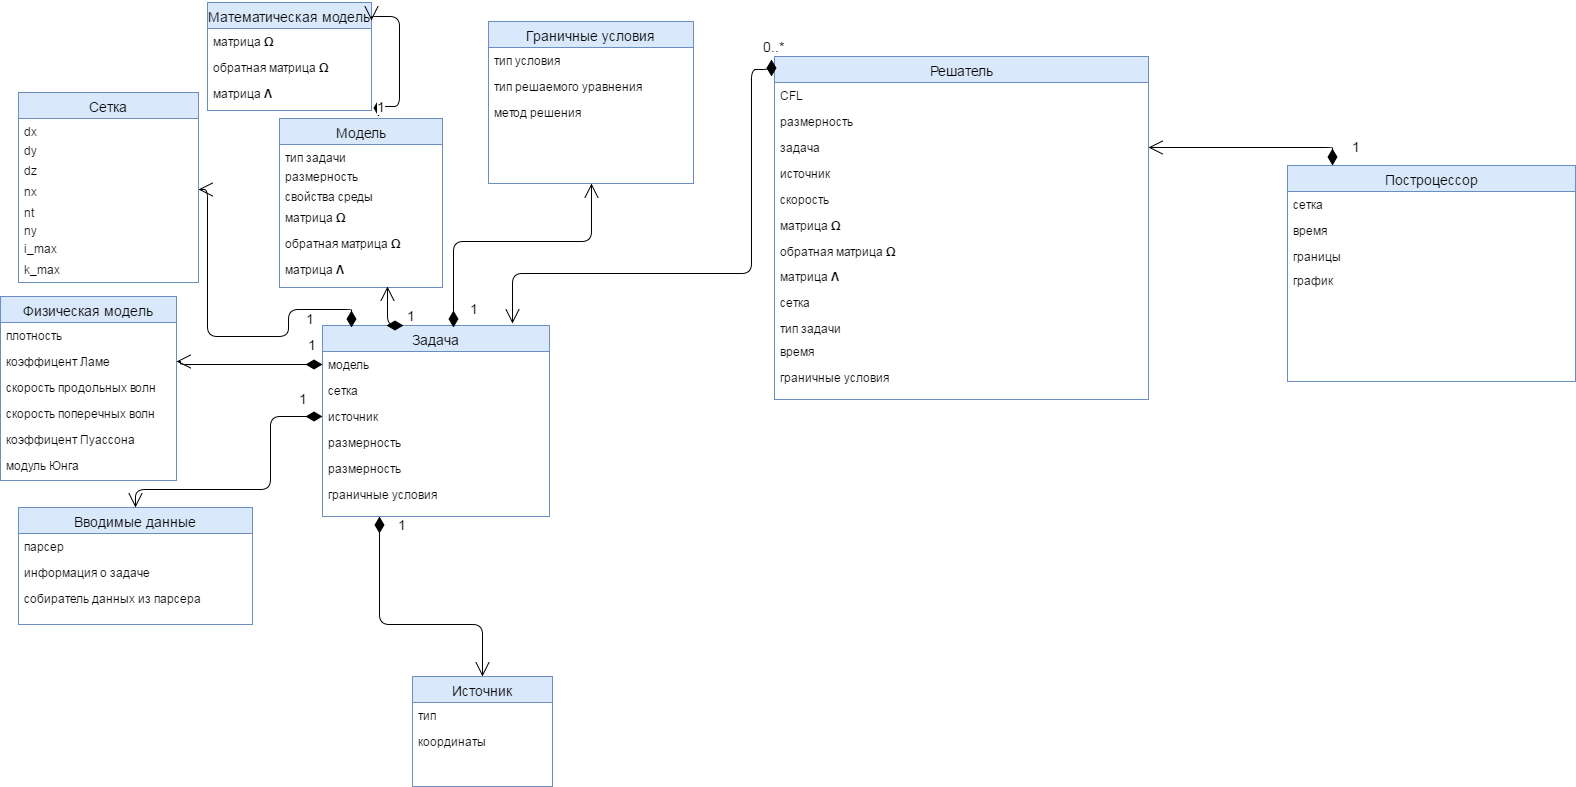
\includegraphics[scale=0.3]{architec.png}
  \end{center}
\end{figure}

\textbf{Описание классов}
\begin{itemize}
\item Вводимые данные

Класс, содержащий в себе парсер, которые собирает вводимые из консоли данные о задаче.
\item Математическая модель

Класс, который содержит в себе информацию о матрицах, необходимых длярешения уравнений акккустики и сейсмики разной размерности.
\item Модель

Класс для задания модели для решения конкретной задачи. Путем анализа вводимых данных, выбирает матрицы из математической модели.
\item Физическая модель

Класс для задания физических свойств среды. Поддерживает задание свойств для гомогенной и гетерогенной сред путем изображения или аналитически.

\item Граничные условия

Класс для задания граничных условий следующих типов: отражение, циклическое, поглощение, приложенная сила, свободная граница.
\item Сетка

Класс для задания сетки решения задачи.
\item Решатель

Получает данные из выше описанных классов, решает задачу соответствующим методом. Считает по времени, применяет граничные условия, применяет источник, разделяет на одномерные задачи, решает их.
\item Постпроцессор

Класс для проверки полученного решения задачи. Содержит в себе методы по визуализации решения.
\end{itemize}

\subsection{Как запустить расчет кейса}

Скачать все файлы с репозитория OpenSAMP, который находится по ссылке https://github.com/pathfinder14/OpenSAPM
Выполнить соответствующие команды:

 python \_\_main\_\_.py path\_to\_file\_with\_problem\_descriptions 

pip install -r requirements.txt
\\
Вся информация о вводимых данных может быть найдена в файле:

/tests/inputs.txt

\section{Тесты}
\subsection{Одномерные уравнения акустики}


 
 
\subsubsection{Test 1: Linear Hyperbolic Equations}

(Finite Volume Methods for Hyperbolic Problems)

Решаем \ref{1D_equs}

Параметры :'$\rho$' = 1.0,  'средняя плотность'

             'K' = 0.25,  'Объемный модуль упругости'
             
             '$\beta$' = 200.,  'Гауссовский параметр ширины'
             
Область: -1 < x < 1
     
Сетка: 800
 
Шаг по времени: $10^{-5}$
 
  Тест взят из библиотека clawpack, \cite{clawpack}
  \href{http://www.clawpack.org/gallery/_static/apps/fvmbook/chap3/acousimple/README.html}{Ссылка на тест}
 
 \begin{figure}[h]
  \begin{center}
    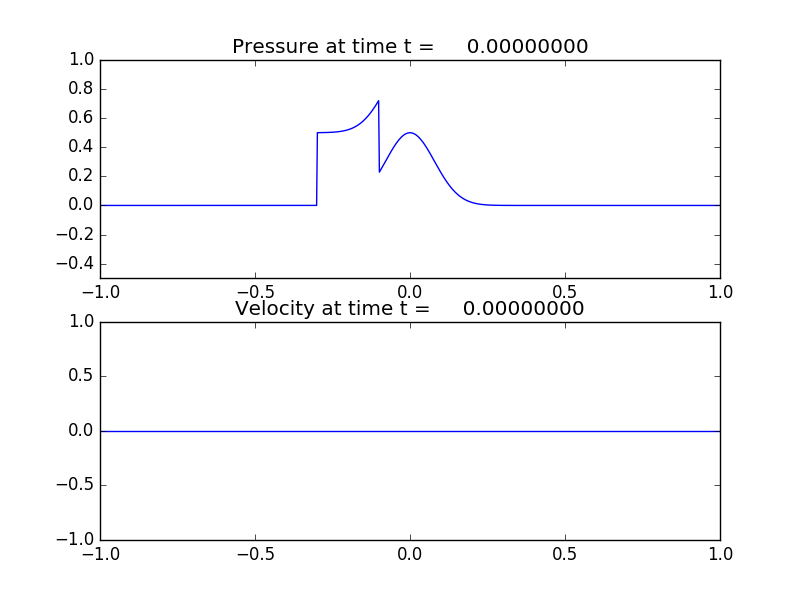
\includegraphics[scale=0.5]{1D_acoustic_test/TEST1/frame0000fig1.png}
  \end{center}
\end{figure}
 
 \newpage
 
\subsubsection{Test 2: Acoustics with a standing wave}

(Акустика с двумя стенами на границах)

Параметры:'$\rho$' = 1.0,  'средняя плотность'

             'K' = 1.0,  'Объемный модуль упругости'
             
             '$\beta$' = 100.,  'начальный импульс'
             
Область: -1 < x < 1
 
Сетка: 200
 
Шаг по времени: $10^{-1}$
 
Координаты стены: x = 0, x = 1
 
  Тест взят из библиотека clawpack, \cite{clawpack}
  \href{http://www.clawpack.org/gallery/_static/apps/fvmbook/chap7/standing/README.html}{Ссылка на тест}
 
 \begin{figure}[h]
  \begin{center}
    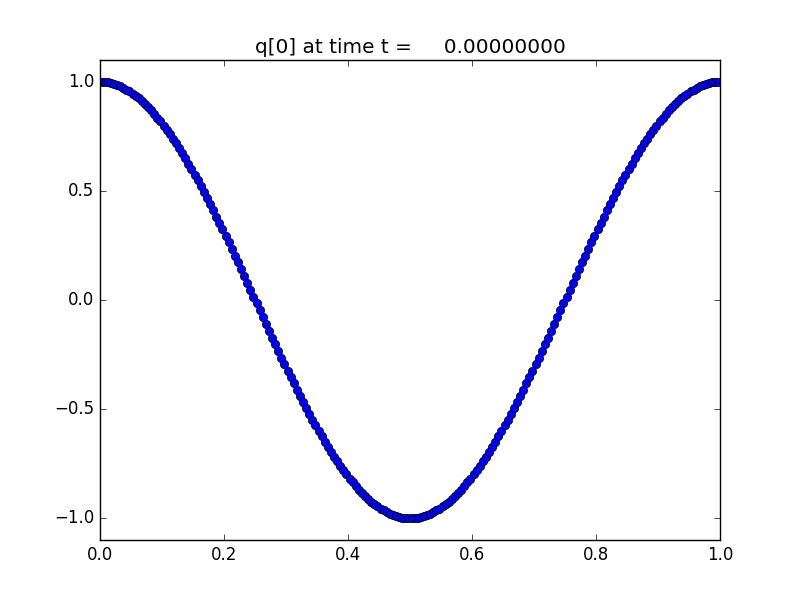
\includegraphics[scale=0.5]{1D_acoustic_test/TEST2/frame0000fig0.png}
  \end{center}
\end{figure}

\newpage
 
 \subsubsection{Test 3}
 
 (Акустика с нулевой инициализацией, волна в x=0, стена в x=1)
 
Ур-ние волны: 0.5*sin($\omega$t)
 
Параметры:'$\rho$' = 1.0,  'средняя плотность'
 
             'K' = 4.0,  'Объемный модуль упругости'
             
             '$\omega$' = 40.,  'параметр омега для начальной волны'
             
Область: -1 < x < 1
 
Сетка: 400
 
Шаг по времени: $10^{-1}$
 
Координаты стены: x = 0, x = 1
 
   Тест взят из библиотека clawpack, \cite{clawpack}
   \href{http://www.clawpack.org/gallery/_static/apps/fvmbook/chap7/acouinflow/README.html}{Ссылка на тест}
   
 \begin{figure}[h]
  \begin{center}
    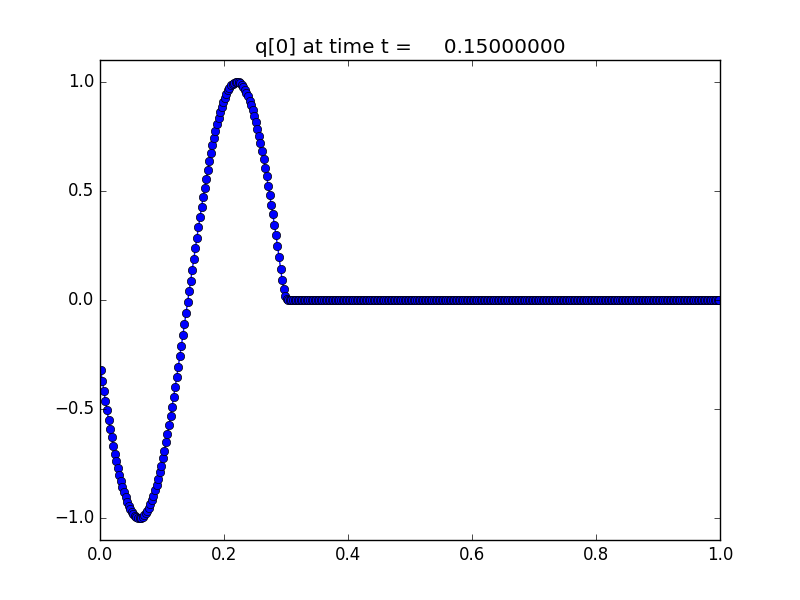
\includegraphics[scale=0.5]{1D_acoustic_test/TEST3/frame0003fig0.png}
  \end{center}
\end{figure}
   
 \subsubsection{Test 4}
Параметры:'$\rho$' = 1.0,  'средняя плотность'

             'K' = 4.0,  'Объемный модуль упругости'
             
             '$\beta$' = 200.,  'начальный импульс'
             
 Area: -1 < x < 1
 
Сетка: 400
 
Шаг по времени: $10^{-1}$
 
Метод: Lax-Wendroff
 
Кол-во волн: 2
 
  Тест взят из библиотека clawpack, \cite{clawpack}
  \href{http://www.clawpack.org/gallery/_static/classic/examples/acoustics_1d_example1/README.html}{Ссылка на тест}
 
 \begin{figure}[h]
  \begin{center}
    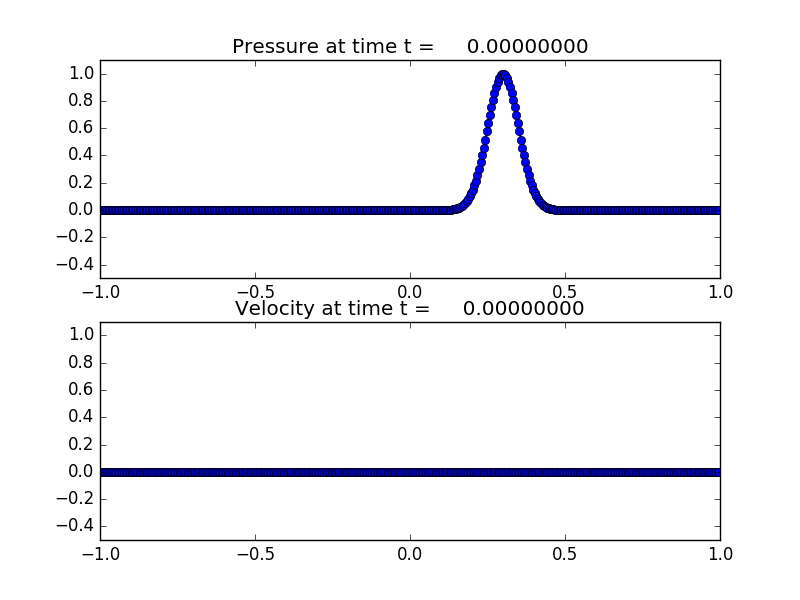
\includegraphics[scale=0.5]{1D_acoustic_test/TEST4/frame0000fig1.png}
  \end{center}
\end{figure}
 
\newpage
\subsection{Двумерные уравнения акустики}

\subsubsection{Тест 1} 

Область: 0 < x < 100 km, 0 < z < 80 km

Шаг: 1 м

Параметры среды: 

$v = 2000 m/s, \rho = 2.3 g/cm^3$ при $z \leq 40 km$

$v = 2300 m/s, \rho = 2.6 g/cm^3$ при $z > 40 km$

Расположение источника: x = 1, z = 40	

Источник:
$$p(t) =  \left[\left(10t  + 0.169^4\right)^{0.25} \cdot 50(10t-0.75)^2 \exp( -15 t) - 4.75\right] \cdot \exp( -10t ) $$

Шаг по времени: 0.2 ms

Выходные данные: давление (p) в зависимости от координат (x, y).

Что должно получиться:

\begin{figure}[h]
  \begin{center}
    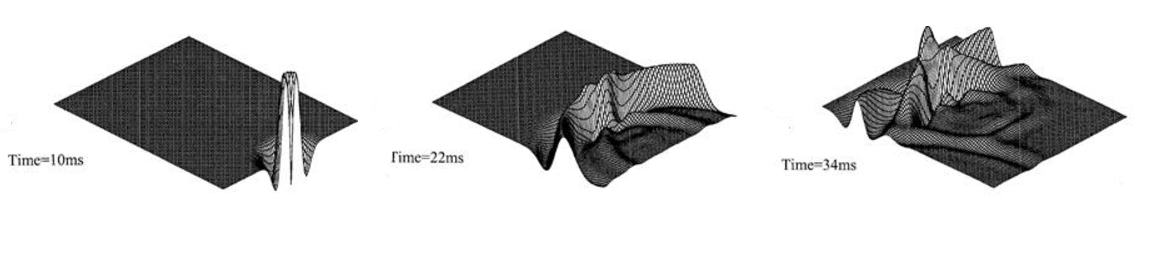
\includegraphics[scale=0.7]{2D_acoustic_tests/second.PNG}
  \end{center}
\end{figure}

Тест взят из \cite{2.5D}

\subsubsection {Распространение гладких акустических волн в 2D} 


Область: -2 < x < 2, -2 < y < 2

Количество точек вдоль одной оси: 5616

Параметры среды:

$ \rho (\overline{x}) = 1$

Расположение источника: (0, 0)

Источник:

$ \overline{v} (\overline{x}, 0) = 0$

$ p(\overline{x}, 0) = 1 + exp(- \alpha r^2)$ , где: $r = \sqrt{x^2 + z^2}$ и $ \alpha = 40$

Что должно получиться:

Численное решение распространения гладкой акустической волны в 2D в момент времени $t = 1.0$. Слева направо: 2D картинка волны в координатах $x$, $y$, цветом показано давление; скорость $u$; давление $p$ и плотность $\rho$.

\begin{figure}[h]
  \begin{center}
    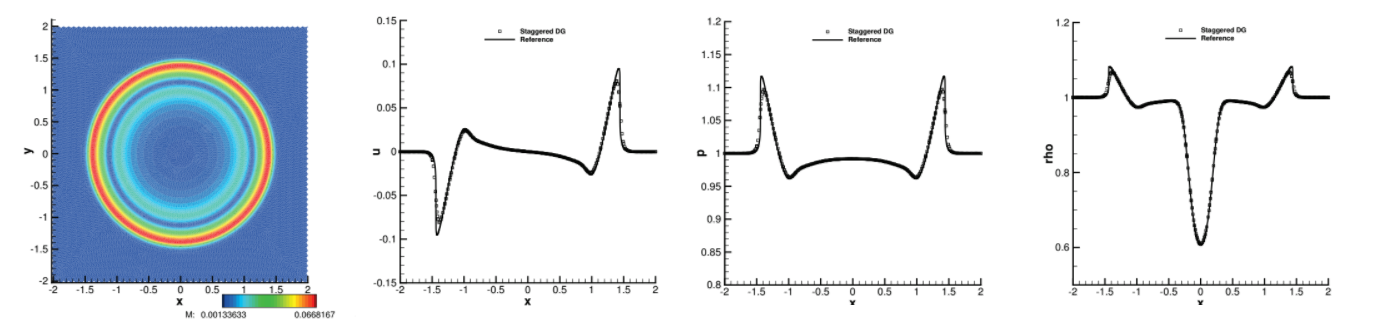
\includegraphics[scale=0.63]{2D_acoustic_tests/third.PNG}
  \end{center}
\end{figure}

Тест взят из \cite{manuscript}

\newpage
\subsection{Одномерные уравнения линейной теории упругости}

\subsubsection{Тест 1}

\begin{wrapfigure}{r}{0.5\textwidth}
  \begin{center}
    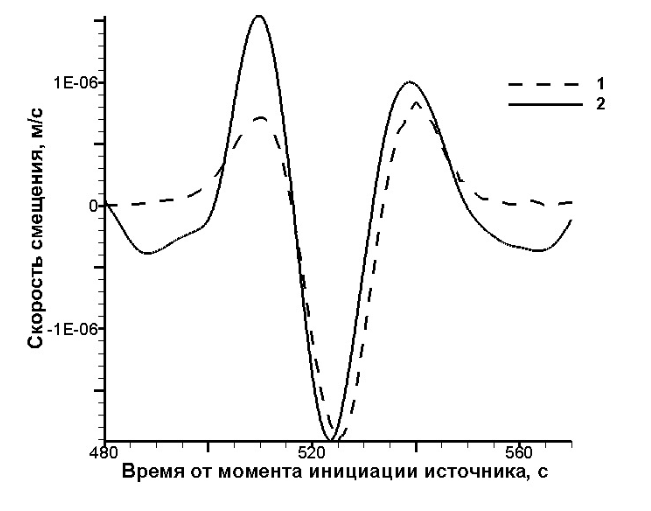
\includegraphics[scale=0.4]{1D_seismic_test/chel.PNG}
  \end{center}
\end{wrapfigure}


Тест взят из \cite{petrov}

Параметры среды: $\rho = 2.6 g/cm^3, {v}_p = 7180 m/s, {v}_s = 3100 m/s;$

($\mu = 24,986 GPa, \lambda = 84,064 GPa$)

Источник точечный.
Физические размер  расчетной области составили $2000\times150 km^3 $

На графике представлено сравнение модельного (1) и реального (2) сигнала.


\newpage
\subsection{Двумерные уравнения линейной теории упругости}

\subsubsection{Тест 1} 

Тест взят из \cite{an_effective}

\begin{wrapfigure}{r}{0.5\textwidth}
  \begin{center}
    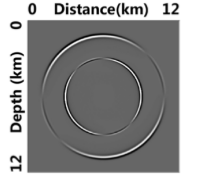
\includegraphics[scale=0.7]{2D_seismic_tests/1.png}
  \end{center}
\end{wrapfigure}


Параметры среды: $\rho = 2.1 g/cm^3, \lambda = 4.704 GPa, \mu = 8.4 GPa$

Область: 0 < x < 12 km, 0 < z < 12 km

Сетка: $400\times400$ (spatial increment 30 m )

Расположение источника: x = 6, z = 6	

Источник: Ricker wavelet
$$f(t) = -5.7 f_0^2\left( 1 - 16 ( 0.6 f_0 t - 1 )^2\right) \cdot \exp\left(-8 ( 0.6 f_0 t - 1 )^2 \right) $$
$$f_0 = 22 Hz$$

Границы: свободные

Шаг по времени: 3 ms

Нужно получить:
\begin{itemize}
\item График распределения модуля скорости $\sqrt{(u^2+w^2)}$ (оси xz) 

\itemГрафик зависимости перемещения от времени в точке R =(6.9, 7.5 km) (для нахождения перемещения, требуется дополнительное интегрирование)
\end{itemize}

Что должно получиться: 

\begin{figure}[h] 
    \begin{subfigure}{0.5\textwidth}
    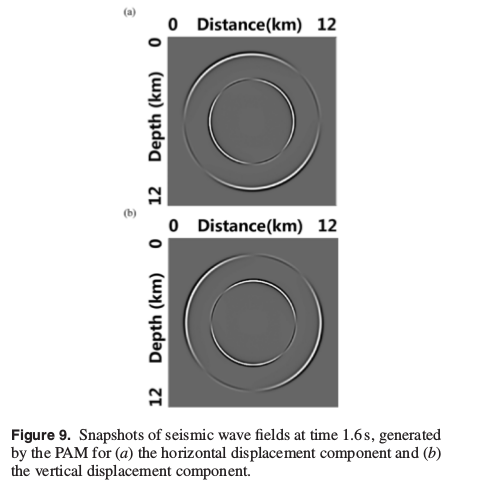
\includegraphics[width=1\linewidth]{2D_seismic_tests/circle1.png} 
    \end{subfigure}
    \begin{subfigure}{0.5\textwidth}
    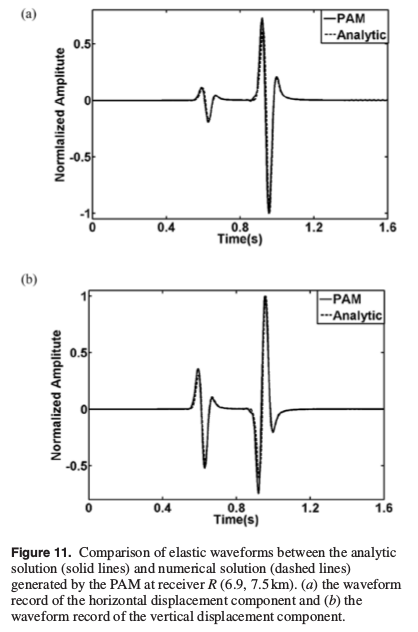
\includegraphics[width=0.7\linewidth]{2D_seismic_tests/circle2.png}
    \end{subfigure}
\end{figure}

% 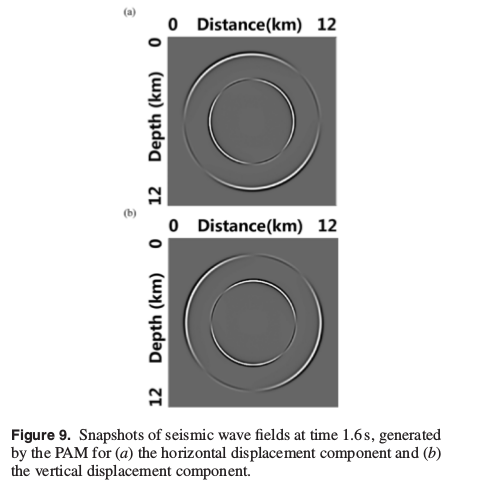
\includegraphics[scale=0.7]{2D_seismic_tests/circle1.png}

% 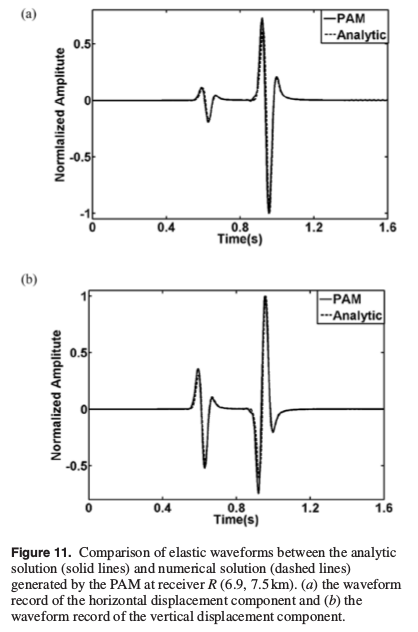
\includegraphics[scale=0.7]{2D_seismic_tests/circle2.png}

\newpage
\subsubsection{Тест 2}

Тест взят из \cite{finite}

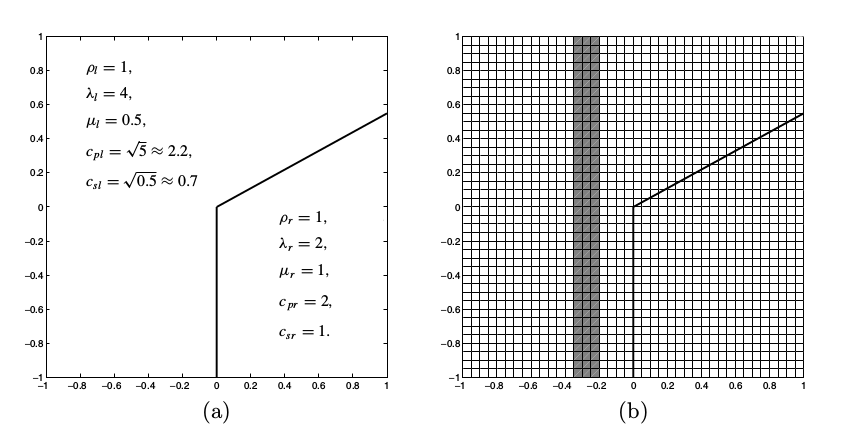
\includegraphics[scale=0.5]{2D_seismic_tests/2.png}

Область: -1 < x < 1, -1 < y < 1

Граница, разделяющая среды:

x = 0, -1 < y < 0

y = 0.55x, 0 < x < 1
		
Начальные условия везде 0, кроме -0.35 < x < -0.2

$\sigma^{11} = \lambda_l+2\mu_l$, $\sigma^{22} = \lambda_l$, $\sigma^{12} = 0, u = c_{pl}, v = 0$

Сетка: $200\times200$

Границы: свободные

Шаг по времени: 0.05

Нужно получить: 

\begin{itemize}
\item График распределения $\sigma^{11}$ (оси xy)

\item График распределения $\sigma^{12}$ (оси xy)

\end{itemize}

Что должно получиться: 

\begin{figure}[h] 
    \begin{subfigure}{0.5\textwidth}
    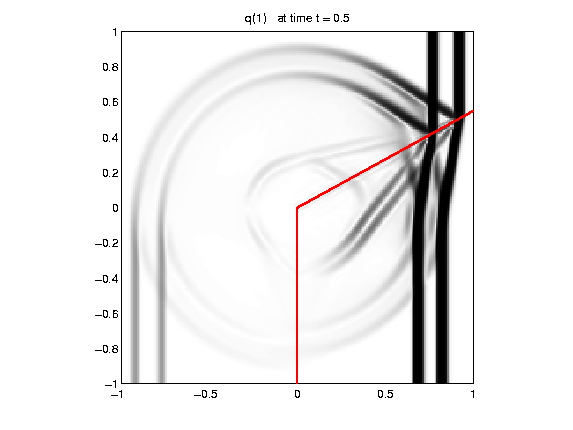
\includegraphics[width=1\linewidth]{2D_seismic_tests/corner-sigma11.png} 
    \end{subfigure}
    \begin{subfigure}{0.5\textwidth}
    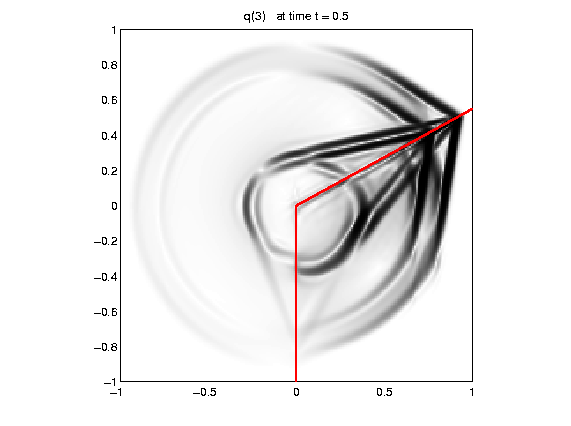
\includegraphics[width=1\linewidth]{2D_seismic_tests/corner-sigma12.png}
    \end{subfigure}
\end{figure}

\newpage
\subsubsection{Тест 3}

Тест взят из \cite{finite}

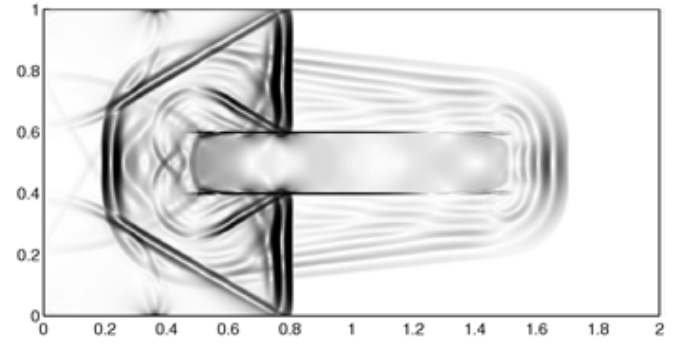
\includegraphics[scale=0.5]{2D_seismic_tests/3.png}

Область: 0 < x < 2, 0 < y < 1

Внешний материал: $ \lambda = 2, \mu = 1, \rho = 1, c_p = 2, c_s = 1$

Внутренний материал: $ \lambda = 200, \mu = 100, \rho = 1, c_p = 20, c_s = 10$

Область внутреннего материала: 0.5 < x < 1.5,  0.4 < y < 0.6

Сетка: $600\times300$

Границы: свободные

Начальные условия:

$u(0,y,t)= 
 \begin{system}
\epsilon sin(\pi t/ 0.025)  if t<0.025 
\\
0 if t > 0.025 
\end{system}$
$v(0,y,t)=0$

Шаг по времени: 0.05

Нужно получить: 

\begin{itemize}
\item График распределения $\sigma^{11}$ (оси xy)

\item График распределения $\sigma^{12}$ (оси xy)

\item График распределения $\sigma^{11} + \sigma^{12}$ (оси xy)

\end{itemize}

Что должно получиться:

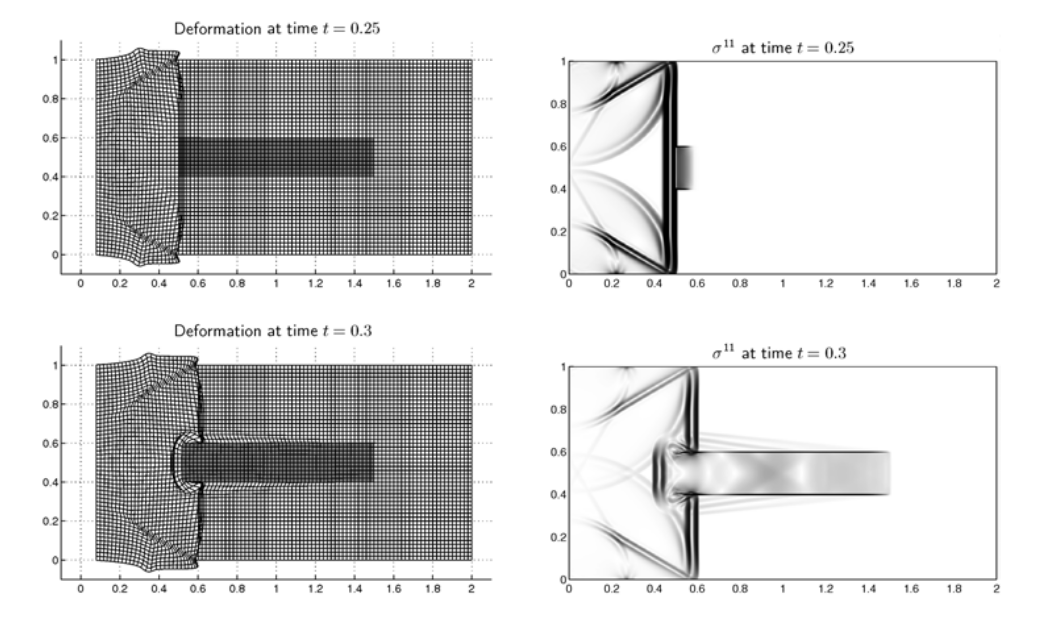
\includegraphics[scale=0.35]{2D_seismic_tests/inclusion1.png}

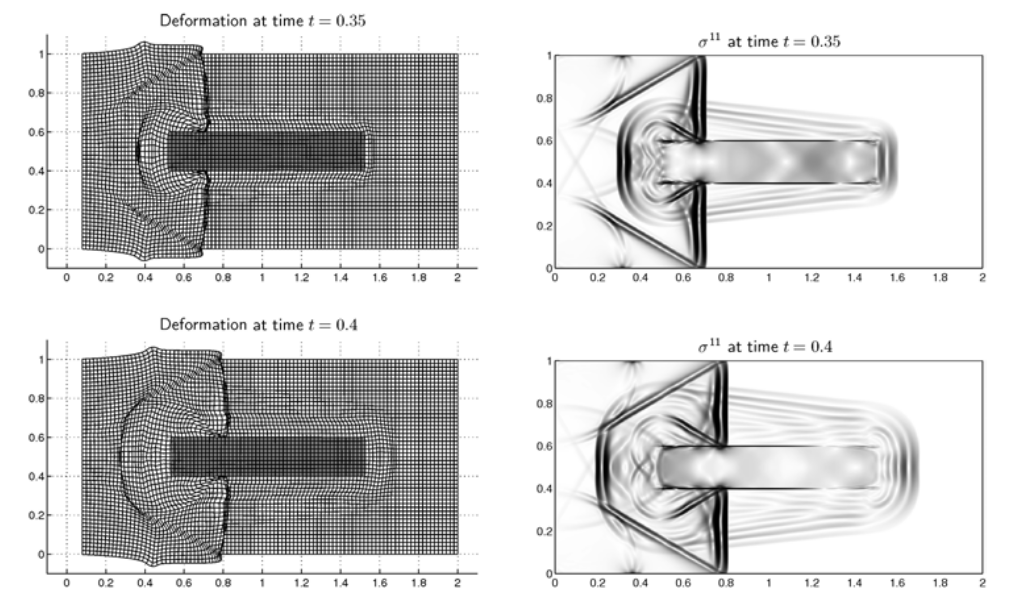
\includegraphics[scale=0.35]{2D_seismic_tests/inclusion2.png}

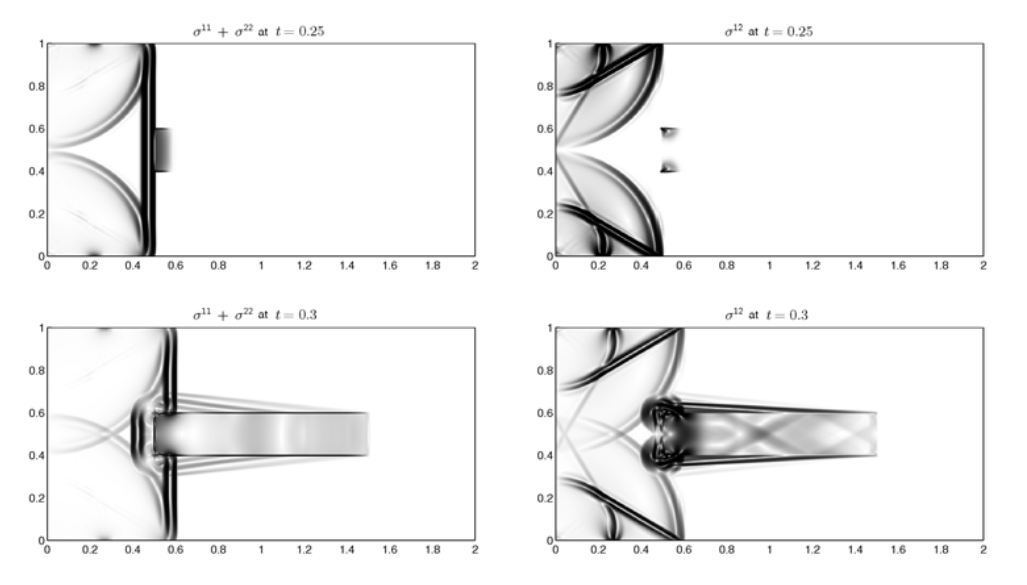
\includegraphics[scale=0.35]{2D_seismic_tests/inclusion3.png}

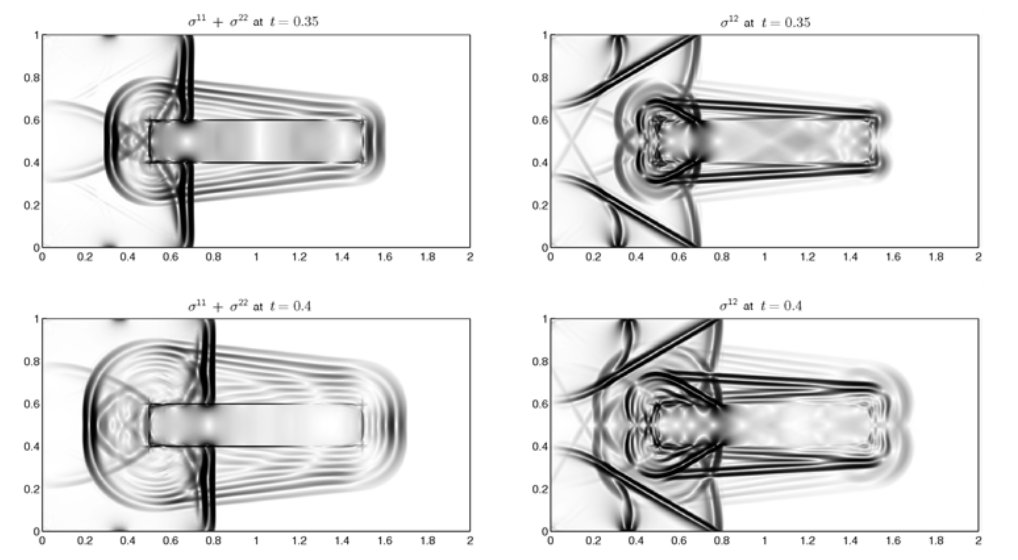
\includegraphics[scale=0.35]{2D_seismic_tests/inclusion4.png}

\newpage
\subsubsection{Тест 4}

Тест взят из \cite{free_and_smooth}

\begin{wrapfigure}{r}{0.5\textwidth}
  \begin{center}
    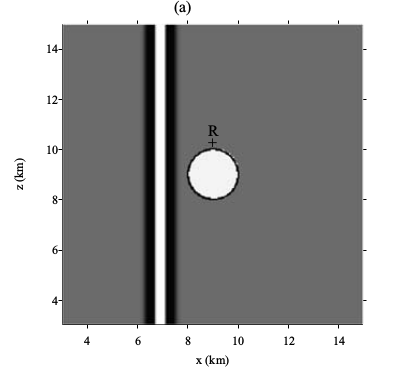
\includegraphics[scale=0.5]{2D_seismic_tests/4.png}
  \end{center}
\end{wrapfigure}

Область: 18x18km

Радиус полости: 1km

Начальные условия: $p~=~2400 kg/m^{-3}$, $c_p~=~4500 m/s^{-1}$, $c_s~=~2200 m/s^{-1}$

Источник: $ g(t) = \left( 2 ( \pi f_c(t - t_c) )^2 - 1 \right) \cdot \exp\left( -\left( \pi f_c(t - t_c)^2 \right) \right)$

$f_{max} = 8 Hz$, $f_{max} \approx 1.6 f_c$, $t_c = 1/f_c$

Сетка: $720\times720$ (h = 25 m)

Границы: свободные

Нужно получить: 

\begin{itemize}
    \item График распределения $v_x$ (оси xz)
\end{itemize}

Что должно получиться:

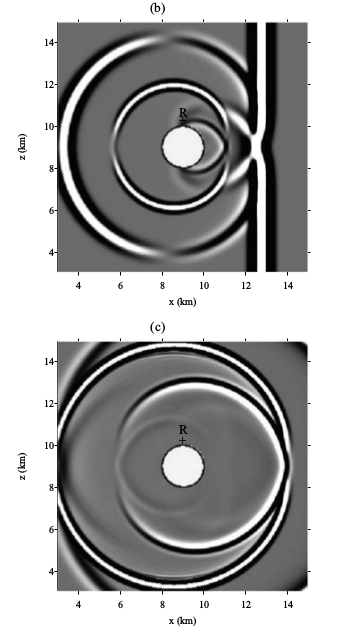
\includegraphics[scale=0.6]{2D_seismic_tests/cavity.png}

\newpage
\subsubsection{Тест 5} 

Тест взят из \cite{chel}

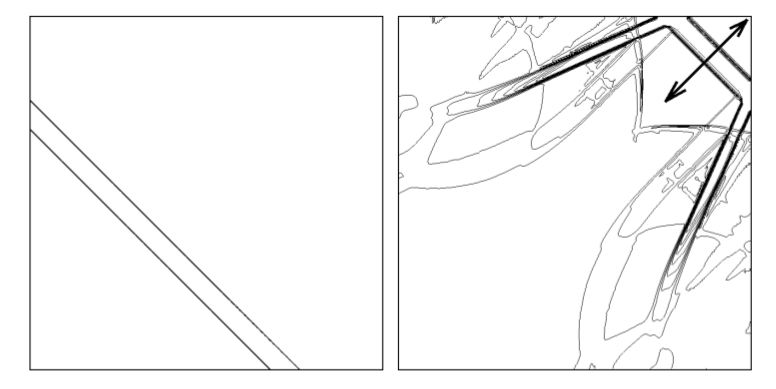
\includegraphics[scale=0.5]{2D_seismic_tests/5.png}

Среда: $\lambda = \mu = 1, \rho = 1$

Область: $[-0.5; 0.5]\times[-0.5; 0.5]$

Начальные условия:
...

Границы: отсутствие внешних сил, отражение

Сетка: $300\times300$

Анализ: на диагонали профиль волны должен сохранить вид ступеньки на момент времени t = 0.4, в который производилось сравнение численных решений. 

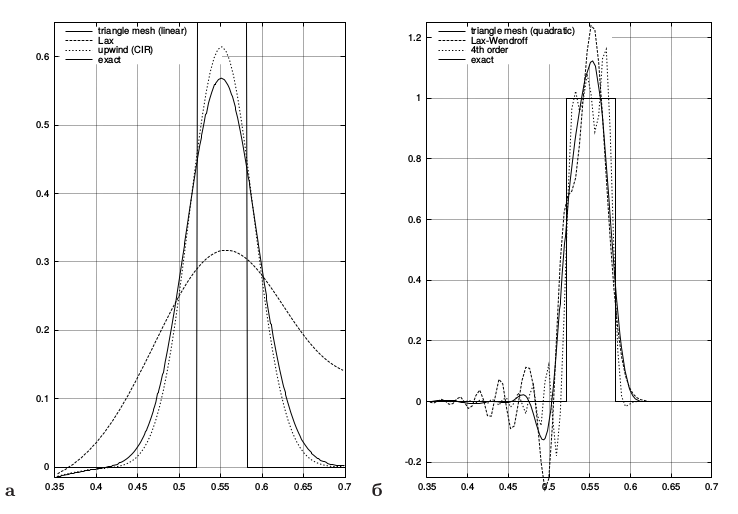
\includegraphics[scale=0.35]{2D_seismic_tests/6.png}

\newpage
\subsubsection{Тест 6}

Аналитическое решение из статьи \cite{garvin}

Среда гомогенная. Граница свободная. Точечный источник (pure P-pulse) на глубине h. Аналитическое решение для y = 0, $-\infty < x < \infty$

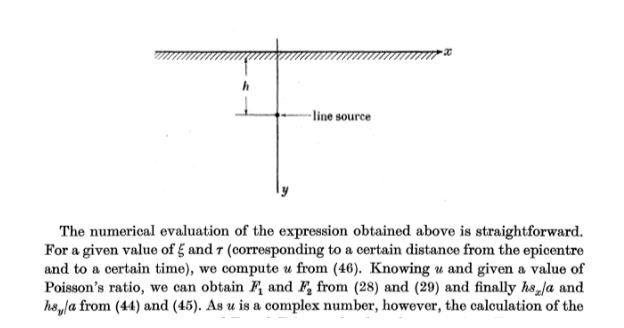
\includegraphics[scale=0.5]{2D_seismic_tests/7.png}

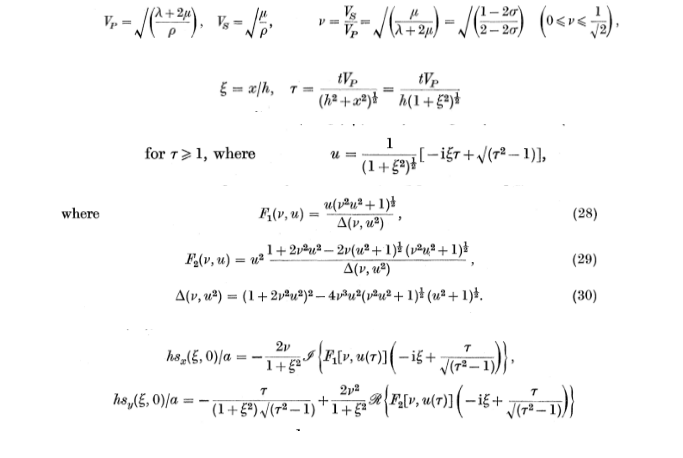
\includegraphics[scale=0.5]{2D_seismic_tests/8.png}

Тест 2 (The Garvin’s problem) из статьи \cite{free_and_smooth}


\newpage
\section{Постпроцессор}
\indent 
Код обильно закомменчен, заинтересованные могут изучить работу подробно. Здесь приведем описание сигнатур методов.

\noindent 
draw1DSlice(solution, t\_slice, x\_start, x\_end, legend, solution\_max\_value, time\_marker\_length) - метод для отрисовки среза по времени, график f(x).
\begin{itemize}
\item solution - одномерный массив, под индексами - сетка по икс, элементы массива - значения сеточной функции в соответствующих узлах
\item t\_slice - время, которое будет отображено в описании графика
\item x\_start - левая граница по икс
\item x\_end - правая страница по икс
\item legend - легенда, будет отображена на описании графика
\item solution\_max\_value - максимальное значение функции на нашей сетке, нужно, чтобы при отрисовке держать границы области по оси ординат постоянными
\item time\_marker\_length - метка, указывающая на длину числа, отображающего время на описании графика
\end{itemize}

\noindent
draw1DMovie(solution, t\_filming\_step, x\_start, x\_end, legend, t\_grid\_step) - метод для рисования мультика по времени. Перед вызовом рисовалки мультика убедитесь, что в конце Draw1DSlice закомменчена строка с выводом изображений и откомменчена строка с сохранением их в папку.
\begin{itemize}
\item solution - двухмерный массив, под первыми индексами - сетка по времени, под вторыми индексами - сетка по икс. Элементы массива - значения сеточной функции в соответствующих узлах.
\item t\_filming\_step - интервалы времени между слайдами, которые мы включаем в гифку, условные секунды
\item x\_start - левая граница по икс
\item x\_end - правая страница по икс
\item legend - легенда, будет отображена на описании графика
\item t\_grid\_step - шаг по временной сетке, условные секунды
\end{itemize}

\noindent 
draw2DSlice(solution, t\_slice, x\_start, x\_end, y\_start, legend, solution\_min\_value, solution\_max\_value, time\_marker\_length) - метод для отрисовки среза по времени, цветовая диаграмма f(x,y).
\begin{itemize}
\item solution - двухмерный массив, под первыми индексами - сетка по иксу, под вторыми индексами - сетка по игрек, элементы массива - значения сеточной функции в соответствующих узлах
\item t\_slice - время, которое будет отображено в описании графика
\item x\_start - левая граница по икс
\item x\_end - правая страница по икс
\item y\_start - нижняя граница нашей области (верхняя всегда 0)
\item legend - легенда, будет отображена на описании графика
\item solution\_max\_value - максимальное значение функции на нашей сетке, нужно, чтобы при отрисовке держать границы цветовой шкалы
\item solution\_min\_value - минимальное значение функции на нашей сетке, нужно, чтобы при отрисовке держать границы цветовой шкалы
\item time\_marker\_length - метка, указывающая на длину числа, отображающего время на описании графика
\end{itemize}

\noindent 
draw1DSliceX(solution, t\_slice, y\_start, y\_end, legend, solution\_max\_value, time\_marker\_length, x\_slice\_value) - служебный метод, не следует вызывать самостоятельно

\noindent
draw1DSliceY(solution, t\_slice, x\_start, x\_end, legend, solution\_max\_value, time\_marker\_length, y\_slice\_value) - служебный метод, не следует вызывать самостоятель


\noindent
draw1DMovieForXSlice(solution, t\_filming\_step, x\_start, x\_end, legend, t\_grid\_step, x\_slice\_value) - служебный метод, не следует вызывать самостоятельно

\noindent
draw1DMovieForYSlice(solution, t\_filming\_step, x\_start, x\_end, legend, t\_grid\_step, y\_slice\_value) - служебный метод, не следует вызывать самостоятельно


\noindent 
\newline
draw2DMovie(solution, t\_filming\_step, x\_start, x\_end, y\_start, legend, solution\_min\_value, solution\_max\_value, t\_grid\_step)
\begin{itemize}
\item solution - трехмерный массив, под первыми индексами - сетка по времени, под вторыми индексами - сетка по икс, под третьими индексами - сетка по игрек, элементы массива - значения сеточной функции в соответствующих узлах
\item t\_filming\_step - интервалы времени между слайдами, которые мы включаем в гифку, условные секунды
\item x\_start - левая граница по икс
\item x\_end - правая страница по икс
\item y\_start - нижняя граница нашей области (верхняя всегда 0)
\item legend - легенда, будет отображена на описании графика
\item solution\_max\_value - максимальное значение функции на нашей сетке, нужно, чтобы при отрисовке держать границы цветовой шкалы
\item solution\_min\_value - минимальное значение функции на нашей сетке, нужно, чтобы при отрисовке держать границы цветовой шкалы
\item time\_marker\_length - метка, указывающая на длину числа, отображающего время на описании графика
\item t\_grid\_step - шаг по сетке по времени
\end{itemize}


section{Свойства среды}
 \indent
Реализованы следующие типы среды, в которой моделируется распространение волн:
\begin{itemize}
\item Гомогенная среда
\item Гетерогенная среда
\end{itemize}
\indent
Среду можно задавать:
\begin{itemize}
\item Изображением:
    \begin{itemize}
    \item Указать путь к картинке, в которой каждому однородному участку среды соответствует свой уникальный цвет.
    \item Задать набор параметров среды для каждого однородного участка (для каждого цвета).
    \end{itemize}
\item Аналитически:
    \begin{itemize}
    \item Указать границы различных слоев среды.
    \item Для каждого слоя указать набор параметров.
    \end{itemize}
\end{itemize}
\indent


\section{Граничные условия}

\indent
Реализованы граничные условия следующих типов:
\begin{itemize}
\item Отражение.
\item Циклическое.
\item Поглощение.
\item Приложенная сила (условие свободной границы является частным случаем этого условия с силой, равной 0).
\end{itemize}

\indent
Метод реализации граничных условий - дополнение расчётной сетки фиктивными узлами.

\indent
Введём для простоты нумерацию узлов дополненной одномерной сетки такой (использована в \cite[глава~7]{finite}): $ \left| Q_{-(l-1)}, ... Q_0 \right| Q_1, ... Q_N \left| Q_{N+1}, ... Q_{N+r} \right|$, где границы находятся посередине между $Q_0$ и $Q_1$ и посередине между $Q_N$ и $Q_{N+1}$ (обозначены вертикальными линиями), $l$ - количество дополненных узлов слева, $r$ - количество дополненных узлов справа.

\indent
Для двумерного случая метод расщепления создаёт одномерные дополняемые сетки, которые обрабатываются аналогично одномерному случаю. Поскольку метод расщепления передаёт функции одномерные сетки по двум перпендикулярным направлениям, а сами элементы сетки имеют составляющие, соответствующие обоим направлениям, для наглядности потребуется ввести индексы направлений. Направление, соответствующая которому координата меняется на сетке, обозначим $main$; направление, перпендикулярное $main$, назовём $extra$.

\subsection{Условие отражения}

\indent
В данном случае для одномерной сетки в необходимое число узлов слева от границы достраивается зеркальная копия ячеек справа от границы, причём значения напряжения берутся того же знака, а значение нормальной скорости умножается на $-1$. То же для правой границы.

\indent
Формальная запись условия слева для одномерного случая сейсмики (слева) и акустики:
$$Q_{-(i-1)} =  \left[ \begin{array}{c}
                      \sigma_i \\
                      -u_i
                      \end{array}    \right] =
                \left[ \begin{array}{c}
                      p_i \\
                      -u_i
                      \end{array}    \right] $$

\indent
Аналогично получается справа:
$$Q_{N+i} = \left[ \begin{array}{c}
                   \sigma_{N+1-i} \\
                   -u_{N+1-i}
                   \end{array}    \right] =
            \left[ \begin{array}{c}
                   p_{N+1-i} \\
                   -u_{N+1-i}
                   \end{array}    \right]$$

\indent
Для случая двумерной акустики условие получается таким:
$$Q_{-(i-1)} =  \left[ \begin{array}{c}
                      p_i \\
                      -u^{main}_{i} \\
                      u^{extra}_{i} 
                      \end{array}    \right] $$

\indent
И, наконец, для двумерной сейсмики:
$$Q_{-(i-1)} =  \left[ \begin{array}{c}
                      \sigma^{main, main}_{i} \\
                      \sigma^{extra, extra}_{i} \\
                      \sigma^{main, extra}_{i} \\
                      -u^{main}_{i} \\
                      u^{extra}_{i}
                      \end{array}    \right] $$

\subsection{Циклическое условие}

\indent
В данном случае для одномерной сетки в необходимое число узлов слева от левой границы записываются без изменений значения в ячейках слева от правой границы \cite[глава 7.1]{finite}. Аналогично для правой границы.

\indent
Формальная запись условия слева для одномерного случая сейсмики (слева) и акустики:
$$Q_{-i} = Q_{N-i} = \left[ \begin{array}{c}
                            \sigma_{N-i} \\
                            u_{N-i}
                            \end{array}    \right] =
                     \left[ \begin{array}{c}
                            p_{N-i} \\
                            u_{N-i}
                            \end{array}    \right] $$

\indent
Аналогично получается справа для сейсмики:
$$Q_{N+i} = Q_{i} = \left[ \begin{array}{c}
                           \sigma_{i} \\
                           u_{i}
                           \end{array}    \right] $$

\indent
Для случая двумерной акустики условие получается таким:
$$Q_{-i} = Q_{N-i} = \left[ \begin{array}{c}
                            p_{N-i} \\
                            u^{main}_{N-i} \\
                            u^{extra}_{N-i} 
                            \end{array}    \right] $$

\indent
И, наконец, для двумерной сейсмики:
$$Q_{-i} = Q_{N-i} = \left[ \begin{array}{c}
                            \sigma^{main, main}_{N-i} \\
                            \sigma^{extra, extra}_{N-i} \\
                            \sigma^{main, extra}_{N-i} \\
                            u^{main}_{N-i} \\
                            u^{extra}_{N-i}
                            \end{array}    \right] $$

\subsection{Условие поглощения}

\indent
В данном случае для одномерной сетки в необходимое число узлов слева от левой границы записываются без изменений значения в зеркально расположенных ячейках справа от границы \cite[глава 7.3.1]{finite}. Аналогично для правой границы.

\indent
Формальная запись условия слева для одномерного случая сейсмики (слева) и акустики:
$$Q_{-(i-1)} = \left[ \begin{array}{c}
                      \sigma_i \\
                      u_i
                      \end{array}    \right] =
               \left[ \begin{array}{c}
                      p_i \\
                      u_i
                      \end{array}    \right] $$

\indent
Аналогично справа для сейсмики:
$$Q_{N+i} = \left[ \begin{array}{c}
                   \sigma_{N+1-i} \\
                   u_{N+1-i}
                   \end{array}    \right] $$

\indent
Для случая двумерной акустики условие получается таким:
$$Q_{-(i-1)} = \left[ \begin{array}{c}
                      p_i \\
                      u^{main}_i \\
                      u^{extra}_i 
                      \end{array}    \right] $$

\indent
И, наконец, для двумерной сейсмики:
$$Q_{-(i-1)} = \left[ \begin{array}{c}
                      \sigma^{main, main}_i \\
                      \sigma^{extra, extra}_i \\
                      \sigma^{main, extra}_i \\
                      u^{main}_i \\
                      u^{extra}_i
                      \end{array}    \right] $$
                  
                  
\subsection{Граничное условие при приложенной силе}

\indent
В данном случае для одномерной сетки в необходимое число узлов слева от левой границы записываются значения в зеркально расположенных ячейках справа от границы \cite[глава 22.4.2]{finite}, причём скорости не изменяются, а значения напряжений или давления меняются по формуле $p = 2 \cdot S - p_{old}$, где $S$ - приложенная к границе сила. Аналогично для правой границы.

\indent
Формальная запись условия слева для одномерного случая сейсмики (слева) и акустики:
$$Q_{-(i-1)} = \left[ \begin{array}{c}
                      2 * S - \sigma_i \\
                      u_i
                      \end{array}    \right] =
               \left[ \begin{array}{c}
                      2 * S - p_i \\
                      u_i
                      \end{array}    \right] $$

\indent
Аналогично справа для сейсмики:
$$Q_{N+i} = \left[ \begin{array}{c}
                   2 * S - \sigma_{N+1-i} \\
                   u_{N+1-i}
                   \end{array}    \right] $$   

\indent
Для случая двумерной акустики условие получается таким:
$$Q_{-(i-1)} = \left[ \begin{array}{c}
                      2 * S - p_i \\
                      u^{main}_i \\
                      u^{extra}_i 
                      \end{array}    \right] $$

\indent
И, наконец, для двумерной сейсмики:
$$Q_{-(i-1)} = \left[ \begin{array}{c}
                      2 * S - \sigma^{main, main}_i \\
                      \sigma^{extra, extra}_i \\
                      2 * S - \sigma^{main, extra}_i \\
                      u^{main}_i \\
                      u^{extra}_i
                      \end{array}    \right] $$


\subsection{Источниковые функции}

\section{Соглашения о структуре и стиле кода}
\subsection{Документирование}

\subsection{Структуры данных}

\subsection{Модули}

\subsection{Функции}

\subsection{Имена переменных}

\subsection{Численные методы}
\subsection{Метод расщепления}

\subsection{КИР, МакКормак, Лакс-Вендрофф, явная схема Бима-Уорминга, явная схема Федоренко,  схема Русанова}

\subsubsection{КИР}

\indent
Разностные уравнения для схемы Куранта-Изаксона-Риса во внутренних точках расчетной области:

$$\frac{u^{n+1}_m - u^n_m}{\tau} + c\frac{u^n_m - u^n_{m-1}}{h} = 0, c > 0$$

$$\frac{u^{n+1}_m - u^n_m}{\tau} + c\frac{u^n_{m+1} - u^n_m}{h} = 0, c < 0$$

\indent
Схема КИР условно устойчива при выполнении условия Куранта $\sigma = c\tau/h \leq 1$.

\begin{figure}[h]
\center{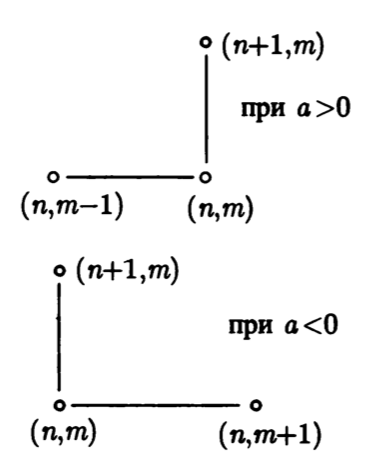
\includegraphics[width=0.2\linewidth]{methods/kir.png}}
\caption{Схема МакКормака}
\label{ris:image}
\end{figure}  

\subsubsection{МакКормак}

\indent
Схема МакКормака состоит из двух этапов. Рассмотрим построение схемы МакКормака для однородного уравнения. Первый этап (предиктор) имеет вид

$$\frac{\tilde{u}^{n}_m - u^n_m}{\tau} + c\frac{u^n_{m+1} - u^n_m}{h} = 0,$$

$$\frac{\tilde{u}^{n}_{m-1} - u^n_m}{\tau} + c\frac{u^n_m - u^n_{m-1}}{h} = 0,$$

т.е. используется схема "явный правый уголок". Второй этап -- корректор:

$$\frac{u^{n+1}_m -0,5(u^n_m + \tilde{u}^m)}{\tau} + c\frac{\tilde{u}^n_{m} - \tilde{u}^n_{m-1}}{2h} = 0.$$

\begin{figure}[h]
\center{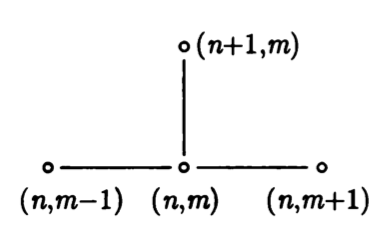
\includegraphics[width=0.3\linewidth]{methods/lax_wendroff.png}}
\caption{Схема МакКормака}
\label{ris:image}
\end{figure}  

\subsubsection{Лакс-Вендрофф}

\indent
Сеточные уравнения для четырёхточечной схемы Лакса-Вендроффа во внутренних узлах расчётных сеток есть

\begin{figure}[h]
\center{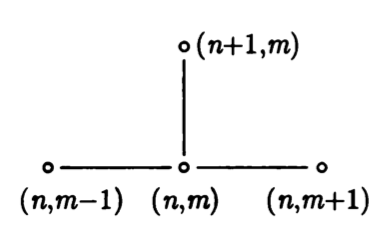
\includegraphics[width=0.3\linewidth]{methods/lax_wendroff.png}}
\caption{Схема Лакса-Вендроффа}
\label{ris:image}
\end{figure}  

$$\frac{u^{n+1}_m - u^n_m}{\tau} + c\frac{u^n_{m+1} - u^n_{m-1}}{2h} - c^2\frac{\tau}{2}\frac{u^n_{m-1} - 2u^n_m + u^n_{m+1}}{h^2} = 0$$

\indent
Порядок апроксимации схемы Лакса-Вендроффа есть $O(\tau^2 + h^2)$. Схема устойчива при выполнении условия Куранта $\sigma = c\tau/h \leq 1$.

\subsubsection{Явная схема Бима-Уорминга}

\indent
Бим и Уорминг предложили изменить метод Мак-Кормака, используя на обоих этапах односторонние разности одинаковой направленности. Разностная схема для явного метода Бима-Уорминга будет

$$u^{n+1}_m = u^n_m - \sigma(u^n_m - u^n_{m-1}) + \frac{\sigma}{2}(1 - \sigma)(u^n_m -2u^n_{m-1} + u^n_{m-2}) = 0$$

\begin{figure}[h]
\center{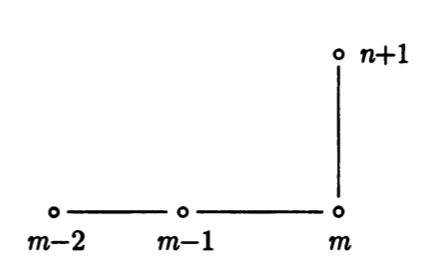
\includegraphics[width=0.3\linewidth]{methods/beam_warming.png}}
\caption{Явная схема Бима-Уорминга}
\label{ris:image}
\end{figure}  

\subsubsection{Явная схема Федоренко}

\indent
Идею построения схемы Федоренко рассмотрим на примере схемы "уголок"

$$L_{\tau}u^{\tau} = \frac{u^{n+1}_{m} - u^{n}_{m}}{\tau} + \frac{u^{n}_{m} - u^{n}_{m-1}}{h} = 0$$

для численного решения модельного уравнения переноса

$$Lu = \frac{\partial u}{\partial t} + \frac{\partial u}{\partial x} = 0.$$

\indent
Разложения сеточных функций проекции на сетку точечного решения дифференциальной задачи в ряд Тейлора дает

$$L_{\tau}u^{\tau} = Lu + \frac{\tau}{2}\cdot \frac{\partial^2 u}{\partial t^2} - \frac{h}{2}\cdot \frac{\partial^2 u}{\partial x^2} + O(\tau^2 + h^2).$$

Полученное выражение может быть представлено в виде разностной схемы

$$\frac{u^{n+1}_{m} - u^{n}_{m}}{\tau} + \frac{u^{n}_{m} - u^{n}_{m-1}}{h} + \frac{1}{2\tau}(\frac{\tau}{h} - \frac{\tau^2}{h^2})(u^n_{m-1} -2u^n_m + u^n_{m+1}) = 0.$$

\begin{figure}[h]
\center{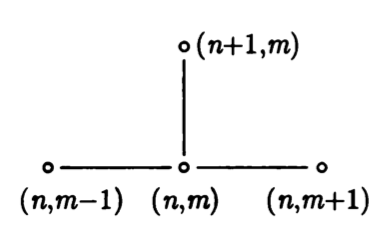
\includegraphics[width=0.3\linewidth]{methods/lax_wendroff.png}}
\caption{Явная схема Федоренко}
\label{ris:image}
\end{figure}  

\subsubsection{Схема Русанова}

\indent
Для построения схемы Русанова вводятся не только полуцелые точки, но и два слоя промежуточных точек с дробными индексами. Первый этап схемы Русанова (переход к слою 1/3) имеет вид

$$\frac{u^{n+1/3}_{m+1/2}-0,5(u^n_m - u^n_{m+1})}{\tau/3} + \frac{f^n_{m+1}-f^n_m}{h} = 0,$$

$$\frac{u^{n+1/3}_{m-1/2}-0,5(u^n_m - u^n_{m-1})}{\tau/3} + \frac{f^n_m-f^n_{m-1}}{h} = 0,$$

ее второй этап есть схема "чехарда"

$$\frac{u^{n+2/3}_{m+1/2}-u^n_m}{2\tau/3} + \frac{f^{n+1/3}_{m+1/2}-f^{n+1/3}_{m-1/2}}{h} = 0,$$

а третий этап

\begin{equation}
\begin{gathered}
\frac{u^{n+1}_{m}-u^n_m}{\tau} + \frac{3}{8}\frac{f^{n+2/3}_{m+1}-f^{n+2/3}_{m-1}}{h}+ \\ + \frac{-2f^n_{m+2} + 7f^n_{m+1} -7f^n_{m-1} + 2f^n_{m-2}}{24h} + \\ + \frac{\omega}{24}(u^n_{m+2} - 4u^n_{m+1} + 6u^n_m - 4u^n_{m-1} + u^n_{m-2}) = 0.
\end{gathered}
\end{equation}

Схема является условно устойчивой при выполнении условия Куранта и условия $4\sigma^2 - \sigma^4 \leq \omega \leq 3.$


\subsection{TVD-схема}

Рассматривается задача Коши для уравнения переноса

$$ \left\{
        \begin{array}{l}
             u_t + au_x = 0\\
             u(0,x) = u_0(x)
        \end{array}
    \right. $$
    
TVD-разностная схема второго порядка точности имеет вид:
$$ u_m^{n+1} = u_m^n - \sigma(f_{m+\frac{1}{2}} - f_{m-\frac{1}{2}}) \: (6.10.1),$$
здесь $\sigma$ - число Куранта:
$$ \sigma = \alpha\tau/h $$
$f_{m+\frac{1}{2}}$ и $f_{m-\frac{1}{2}}$ - антидиффузионные потоки:
$$ f_{m+\frac{1}{2}} = u_m^n + \frac{1}{2} \phi( r_m ) \cdot ( 1 - \sigma ) \cdot ( u_{m+1}^n - u_m^n ) \: (6.10.2)$$
$$ f_{m-\frac{1}{2}} = u_{m-1}^n + \frac{1}{2} \phi( r_{m-1} ) \cdot ( 1 - \sigma ) \cdot ( u_m^n - u_{m-1}^n ) \: (6.10.3)$$

Функция $\phi(r_m)$ называется лимитером. Параметр $r_m$ вычисляется по формуле:
$$ r_m = \frac{u_m - u_{m-1}}{u_{m+1} - u_m} \: (6.10.4).$$

Приведем лимитеры, примененные в работе:

Superbee:

$$\phi_{sb}(r) = max[0, min(2r,1),min(r,2)] \: (6.10.5).$$

Monotonized central:

$$\phi_{mc}(r) = max[0, min(2r,0.5(1+r),2)]; \: \lim\limits_{r\to \infty}\phi_{mc}(r) = 2 \: (6.10.6). $$

Minmod:

$$ \phi_{mm}(r) = max[0, min(1,r)]; \: \lim\limits_{r\to \infty}\phi_{mm}(r) = 1  \: (6.10.7). $$

Koren:

$$\phi_{kn}(r) = max[0, min(2r,(1 + 2r)/3,2)]; \: \lim\limits_{r\to \infty}\phi_{kn}(r) = 2 \: (6.10.8). $$

Osher:

$$\phi_{os}(r) = max[0, min(r, \beta)], \: (1\leq\beta\leq2); \: \lim\limits_{r\to \infty}\phi_{os}(r) = \beta \: (6.10.9). $$

Ospre:

$$\phi_{op}(r) = \frac{1.5(r^2 + r)}{(r^2 + r + 1}; \: \lim\limits_{r\to \infty}\phi_{op}(r) = 1.5 \: (6.10.10). $$

Smart:

$$\phi_{sm}(r) = max[0, min(2r,(0.25+0.75r),4)]; \: \lim\limits_{r\to \infty}\phi_{sm}(r) = 4 \: (6.10.11). $$

Sweby:

$$\phi_{sw}(r) = max[0, min({\beta}r,1), min(r, \beta)], \: (1\leq\beta\leq2); \: \lim\limits_{r\to \infty}\phi_{sw}(r) = \beta \: (6.10.12). $$

Van Albada 1:

$$\phi_{va1}(r) = \frac{r^2 + r}{r^2 + 1}; \: \lim\limits_{r\to \infty}\phi_{va1}(r) = 1 \: (6.10.13). $$

UMIST:

$$\phi_{um}(r) = max[0, min(2r,(0.25 + 0.75r),(0.75+0.25r),2)]; \: \lim\limits_{r\to \infty}\phi_{um}(r) = 2 \: (6.10.14). $$

Van Albada 2:

$$\phi_{va2}(r) = \frac{2r}{r^2 + 1}; \: \lim\limits_{r\to \infty}\phi_{va2}(r) = 0 \: (6.10.15). $$

Van Leer:

$$\phi_{vl}(r) = \frac{r + |r|}{1 + |r|}; \: \lim\limits_{r\to \infty}\phi_{vl}(r) = 2 \: (6.10.16). $$

\newpage
Рассмотрим результаты, полученные с помощью лимитера Monotonized central.
\begin{figure}[h]
    \caption{Ступенька}
    \begin{subfigure}{0.33\textwidth}
    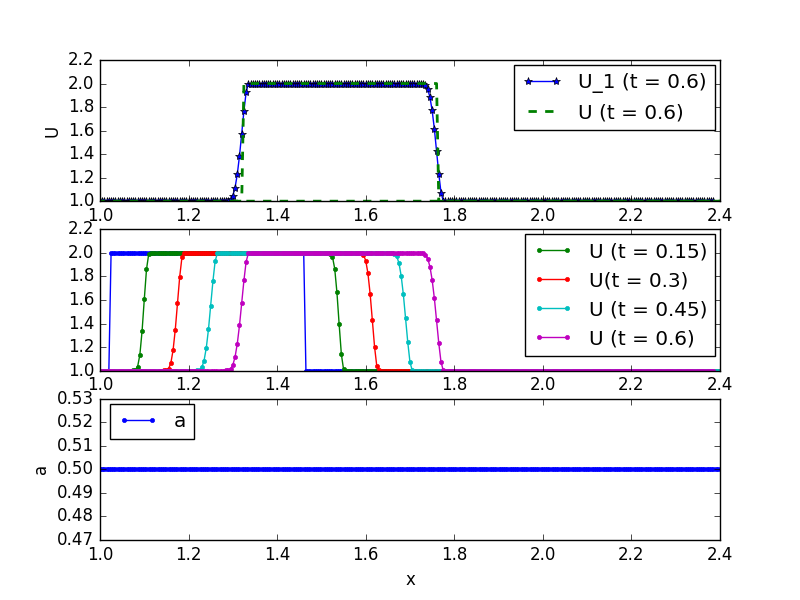
\includegraphics[width=1\linewidth]{TVD_tests/lim_MC_a_const_U0_step.png}
    \end{subfigure}
    \begin{subfigure}{0.33\textwidth}
    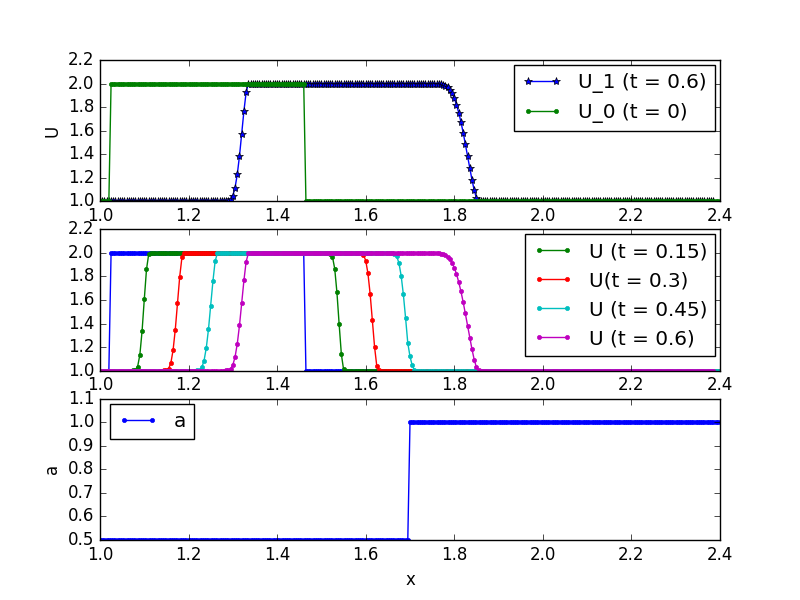
\includegraphics[width=1\linewidth]{TVD_tests/lim_MC_a_devided_U0_step.png}
    \end{subfigure}
    \begin{subfigure}{0.33\textwidth}
    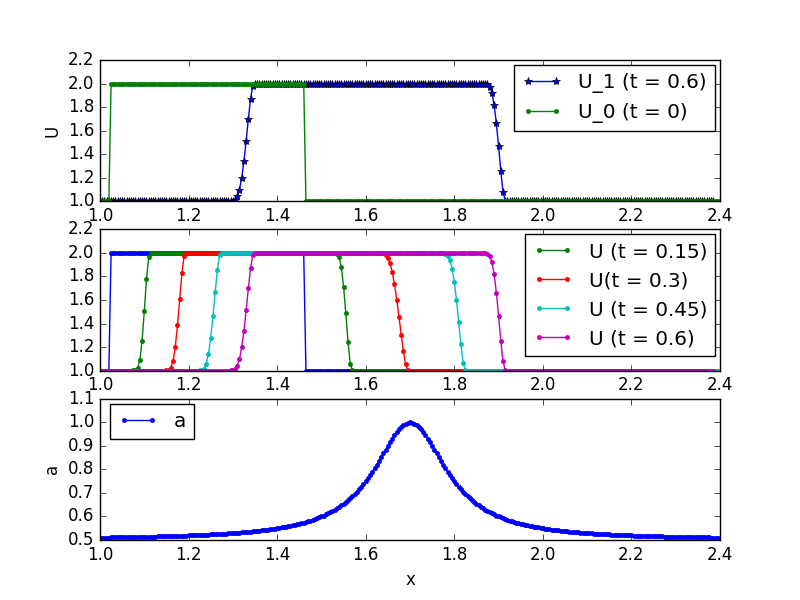
\includegraphics[width=1\linewidth]{TVD_tests/lim_MC_a_hat_U0_step.png}
    \end{subfigure}
\end{figure}
\begin{figure}[h]
    \caption{Гауссиан}
    \begin{subfigure}{0.33\textwidth}
    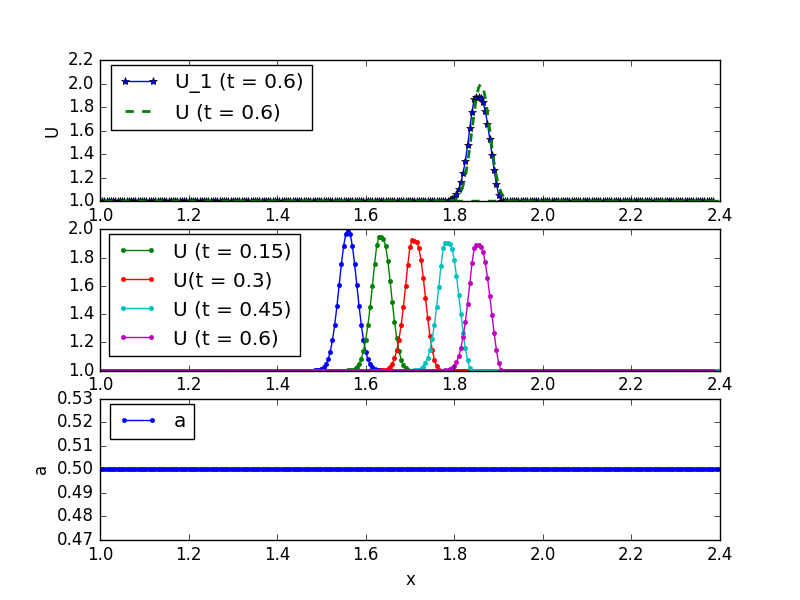
\includegraphics[width=1\linewidth]{TVD_tests/lim_MC_a_const_U0_gauss.png}
    \end{subfigure}
    \begin{subfigure}{0.33\textwidth}
    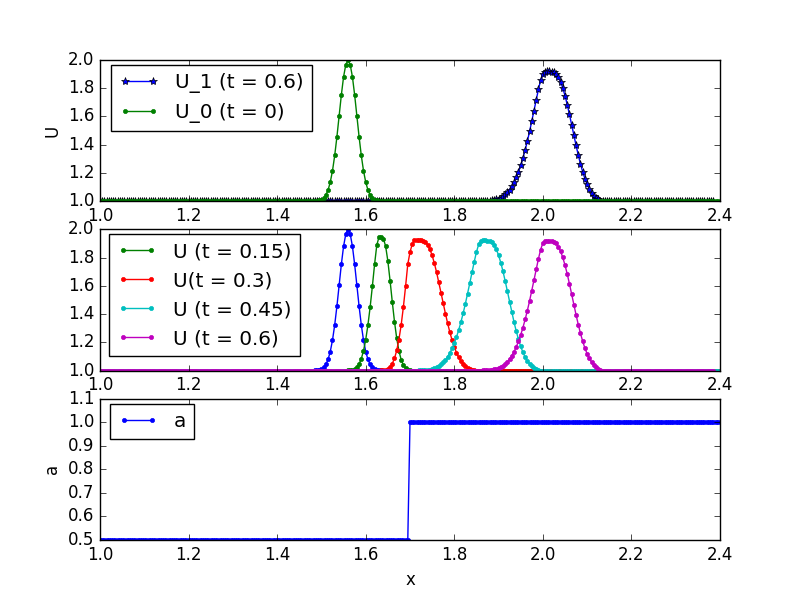
\includegraphics[width=1\linewidth]{TVD_tests/lim_MC_a_devided_U0_gauss.png}
    \end{subfigure}
    \begin{subfigure}{0.33\textwidth}
    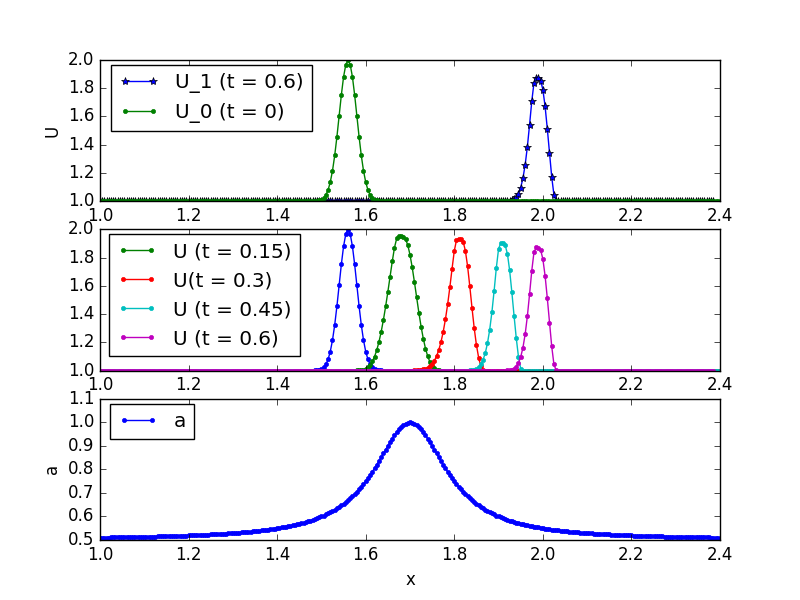
\includegraphics[width=1\linewidth]{TVD_tests/lim_MC_a_hat_U0_gauss.png}
    \end{subfigure}
\end{figure}
\begin{figure}[h]
    \caption{Пик}
    \begin{subfigure}{0.33\textwidth}
    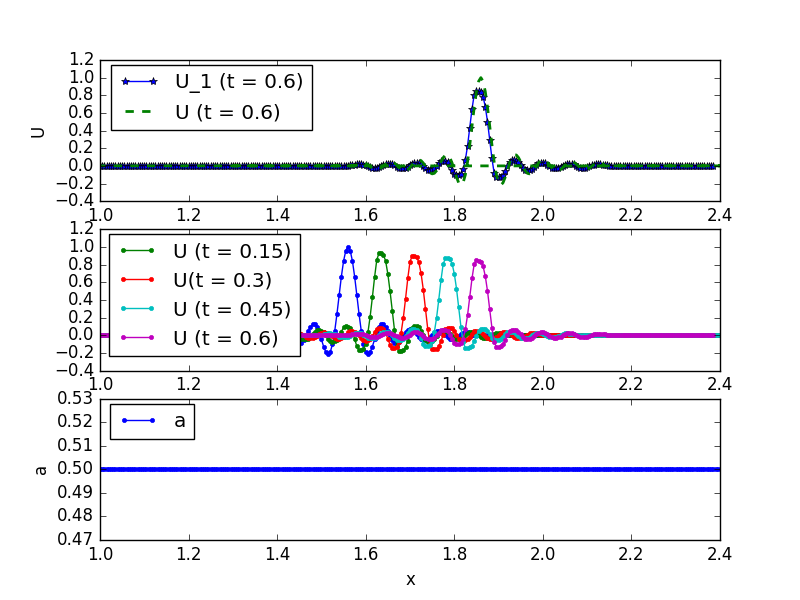
\includegraphics[width=1\linewidth]{TVD_tests/lim_MC_a_const_U0_peack.png}
    \end{subfigure}
    \begin{subfigure}{0.33\textwidth}
    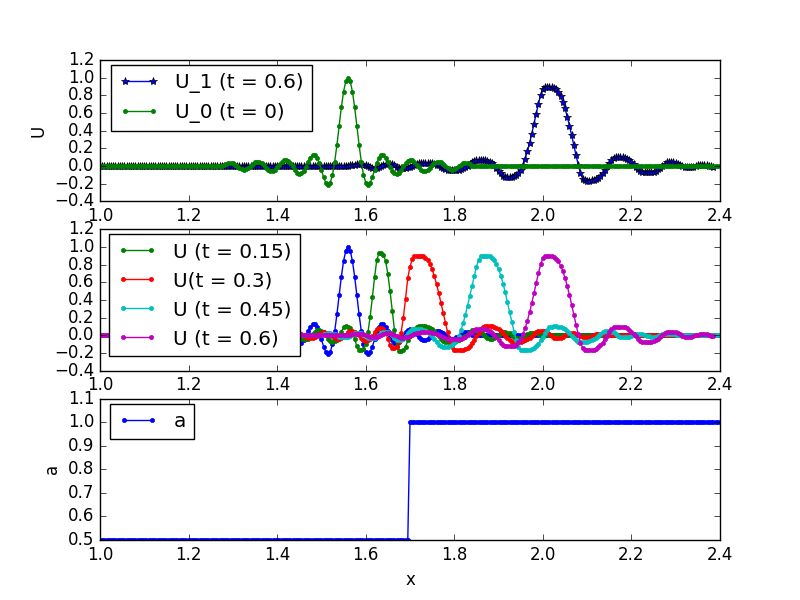
\includegraphics[width=1\linewidth]{TVD_tests/lim_MC_a_devided_U0_peack.png}
    \end{subfigure}
    \begin{subfigure}{0.33\textwidth}
    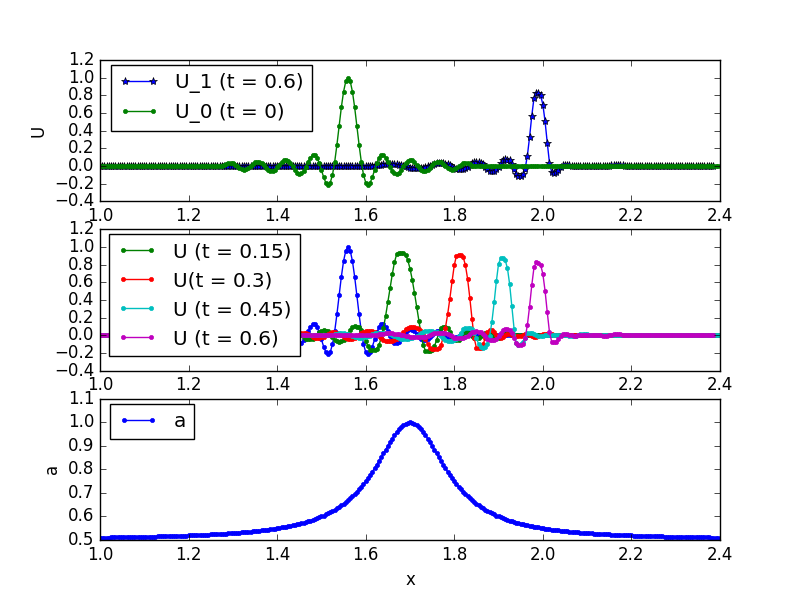
\includegraphics[width=1\linewidth]{TVD_tests/lim_MC_a_hat_U0_peack.png}
    \end{subfigure}
\end{figure}


\subsection{Схема WENO}

Стандартные TVD-схемы хорошо подходят для сверхзвуковых течений с небольшим числом изолированных ударных волн. Однако, задачи, содержащие многочисленные сложные структуры в областях, где решение гладкое, требует более точных вычислительных инструментов. Одним из таких является WENO схемы. В схемах WENO вместо выбора одного из допустимых шаблонов используется их выпуклая линейная комбинация с коэффициентами,
зависящими от решения.
Рассмотрим схему WENO 5-го порядка аппроксимации, использующую три
разностных шаблона (рис.3).
\begin{figure}[h]
\center{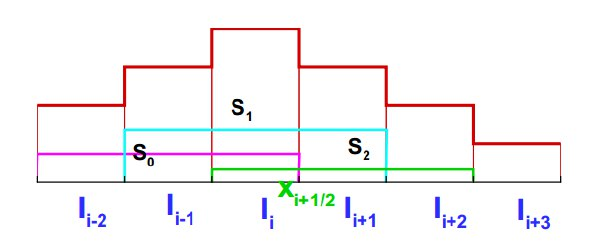
\includegraphics[width=0.7\linewidth]{methods/weno5d.jpg}}
\caption{Шаблоны схемы WENO 5-го порядка}
\label{ris:image}
\end{figure}

Поток через грань $F_{i+1/2}$ вычисляется с помощью точного или
приближенного решения задачи о распаде разрыва между состояниями $u^L_{i+1/2}, \: u^R_{i+1/2}: \: F_{i+1/2} = \: F(u^L_{i+1/2},u^R_{i+1/2})$,

где $u^L_{i+1/2},u^R_{i+1/2}$ - параметры на двух сторонах грани между ячейками.
Выражение для $u^L_{i+1/2}$ дается формулами:
$$u^L_{i+1/2} = w_1v_1 + w_2v_2 + w_3v_3 $$
где $v_k$ - экстраполированное значение:
$$v_1 = \frac{1}{6}(-u_{i+2} + 5u_{i+1} + 2u_i)$$
$$v_2 = \frac{1}{6}(-u_{i-1} + 5u_i + 2u_{i+1})$$
$$v_3 = \frac{1}{6}(2u_{i-2} - 7u_{i-1} + 11u_i)$$
где $w_k$ - веса линейной комбинации.

В общем случае, в области гладкого решения можно построить линейную комбинацию из всех трех шаблонов с оптимальными весами, получив 5-й порядок аппроксимации по пространству. В области гладкого решения веса должны быть близки к оптимальным. В нашем случае $C_1 = 3/10, C_2 = 6/10, C_3 = 1/10.$ Окончательное выражение для весов:
$$w_k = \frac{\alpha_k}{\alpha + \alpha_2 + \alpha_3}, $$
$$\alpha_k = \frac{C_k}{(\epsilon + IS_k)^2}, $$
$$IS_k = \int\limits_{x_{i-1/2}}^{x_{i+1/2}} [\Delta x(\frac{\partial p_k}{\partial x})^2 + \Delta x^3(\frac{\partial^2 p_k}{\partial x^2})^2]dx,$$
где $p_k(x)$ - соответствующий интерполляционный полином.

Для каждого шаблона индикаторы гладкости:
$$IS_1 = \frac{13}{12}(u_i - 2u_{i+1} + u_{i+2})^2 + \frac{1}{4}(3u_i - 4u_{i+1} + u_{i+2})^2, $$
$$IS_2 = \frac{13}{12}(u_{i-1} - 2u_i + u_{i+1})^2 + \frac{1}{4}(u_{i-1} - u_{i+1})^2, $$
$$IS_3 = \frac{13}{12}(u_{i-2} - 2u_{i-1} + u_{i})^2 + \frac{1}{4}(u_{i-2} - 4u_{i-1} + u_i)^2. $$

Для конечнообъемных схем:

1. Используя WENO реконструкцию получить величины $u^L_{i+1/2}$ и $u^R_{j+1/2}$;

2. Вычислить потоки $F_{i+1/2}$, решая задачу о распаде разрыва на гранях между ячейками;

3. Проинтегрировать по времени уравнение:
$$\frac{dU_i}{dt} = -\frac{1}{\Delta x}(F_{j+1/2} - F_{j-1/2}).$$

Для более подробного изучения теории WENO-схем следут ознакомиться с литературой [9],[10].




\subsection{Бикомпактная схема}

Рассматривается задача Коши для гиперболического уравнения
$$  \left\{
        \begin{array}{l}
            u_t + f(u)_x = 0 \\
            u(x,0) = u_0(x), \: x\geq0 \\
            u(0,t) = \mu(t), \: t>0
        \end{array}
    \right. $$

После ряда преобразований получим систему из двух разностных уравнений:
$$  \left\{
        \begin{array}{l}
            \frac{1}{6}(u_{j+1}+4u_{j+1/2}+u_j)_t = -\frac{1}{h}[f(u_{j+1})-f(u_j)], \: j \geq 0 \\
            \frac{h}{4}(u_{j+1}-u_j)_t = -[f(u_{j+1})-2f(u_{j+1/2})+f(u_j)], \: j \geq 0
        \end{array}
    \right. $$
где $u_j, \: u_{j+1}$ - значения искомой функции в целых узлах, $u_{j+1/2}$ - значение в половинном узле. $h$ - шаг сетки по пространственной координате.

В нашем случае $f(u)=au,\:a=const$.
$$  \left\{
        \begin{array}{l}
            \frac{1}{6}(u_{j+1}+4u_{j+1/2}+u_j)_t = -\frac{a}{h}[u_{j+1}-u_j], \: j \geq 0 \\
            \frac{h}{4}(u_{j+1}-u_j)_t = -a[u_{j+1}-2u_{j+1/2}+u_j], \: j \geq 0
        \end{array}
    \right. $$

Заменим производную по времени разностной схемой первого порядка
$$\frac{1}{6}(u^{n+1}_{j+1}+4u^{n+1}_{j+1/2}+u^{n+1}_j)+ar[u^n_{j+1}-u^n_j] = \frac{1}{6}(u^n_{j+1}+4u^n_{j+1/2}+u^n_j), \: j\geq0, $$
$$\frac{1}{4}(u^{n+1}_{j+1}-u^{n+1}_j) + ar[u^n_{j+1}-2u^n_{j+1/2}+u^n_j] = \frac{1}{4}(u^n_{j+1}-u^n_j), \: j\geq0.$$
где $r=\frac{\tau}{h}$, $\tau$ - шаг сетки по времени.

В итоге мы получаем четырехточечную схему, имеющую четвертый порядок аппроксимации по пространственной координате и первый порядок по времени.

Используя начальные и граничные условие, мы можем решить данную систему относительно двух неизвестных переменных $u^{n+1}_{j+1}$ и $u^{n+1}_{j+1/2}$.


\begin{figure}[h]
    \begin{minipage}[h]{0.49\linewidth}
        \center{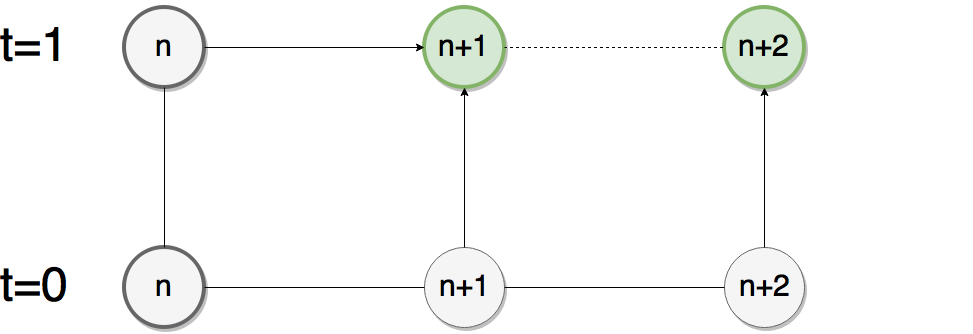
\includegraphics[width=1\linewidth]{methods/bicompact_left.png} \\$a>0$}
    \end{minipage}
    \hfill
    \begin{minipage}[h]{0.49\linewidth}
        \center{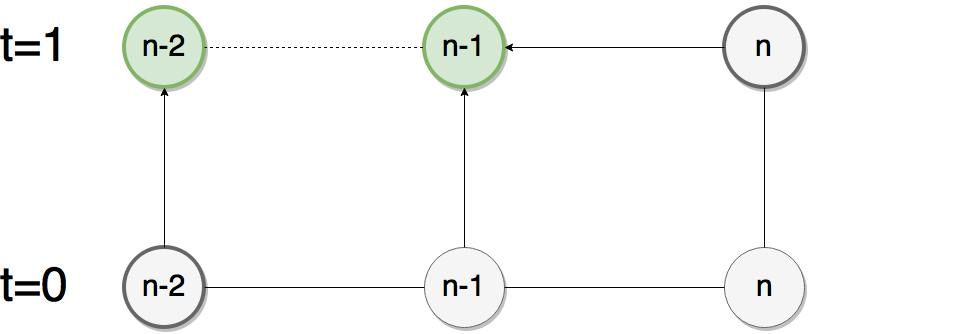
\includegraphics[width=1\linewidth]{methods/bicompact_right.png} \\$a<0$}
    \end{minipage}
    \caption{Шаблон бикомпактной схемы}
    \label{ris:image1}
\end{figure}

В нашем случае, когда начальные значения половинных узлов неизвестны, мы можем, увеличив шаг вдвое, использовать данный шаблон на целых узлах $j,j+1,j+2$.

Для того, чтобы задать граничные условия, используется явный метод, полученный методом неопределенных коэффицентов.
$$\frac{1}{\tau}(u^{n+1}_j-u^{n}_j)=\frac{1}{h}(Au^{n}_j+Bu^{n}_{j+1}+Cu^{n}_{j+2}+Du^{n}_{j+4}) $$
$$A=\frac{11}{6},\:B=-3,\:C=\frac{3}{2},\:D=-\frac{1}{3}$$

\begin{figure}[h]
\center{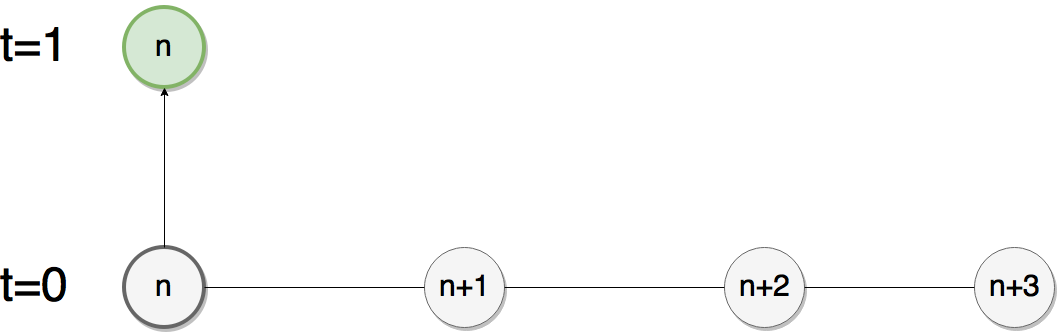
\includegraphics[width=0.7\linewidth]{methods/bicompact_border.png}}
\caption{Шаблон для нахождения граничного условия}
\label{ris:image}
\end{figure}  

\newpage
\subsubsection{Тесты для бикомпактной схемы}

Тесты проводились при исходном сигнале вида "ступенька" , "пик" и вида гауссового распределения, а так же при постоянном значении параметра $a$, разрывного $a$ и $a$ вида "шляпка". 

\begin{figure}[h]
    \caption{Ступенька}
    \begin{subfigure}{0.33\textwidth}
    {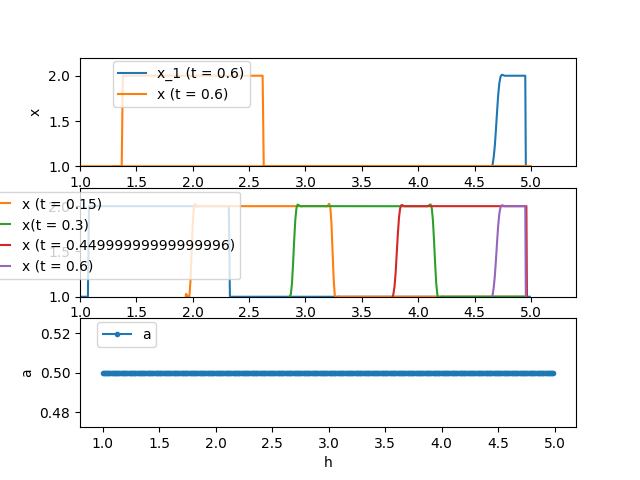
\includegraphics[width=1\linewidth]{tests_bcomp/a_const_x0_step.png} \\$a=const$}
    \end{subfigure}
    \begin{subfigure}{0.33\textwidth}
    {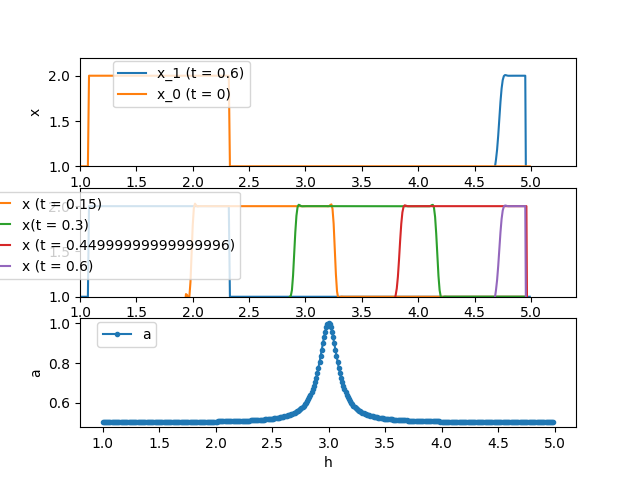
\includegraphics[width=1\linewidth]{tests_bcomp/a_hat_x0_step.png} \\$a - hat$}
    \end{subfigure}
    \begin{subfigure}{0.33\textwidth}
    {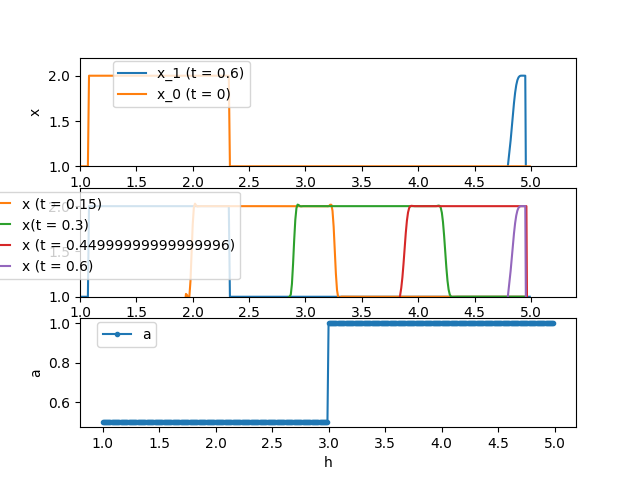
\includegraphics[width=1\linewidth]{tests_bcomp/a_tear_x0_step.png} \\$a - tear$}
    \end{subfigure}
\end{figure}
\begin{figure}[h]
    \caption{Гауссиан}
    \begin{subfigure}{0.33\textwidth}
    {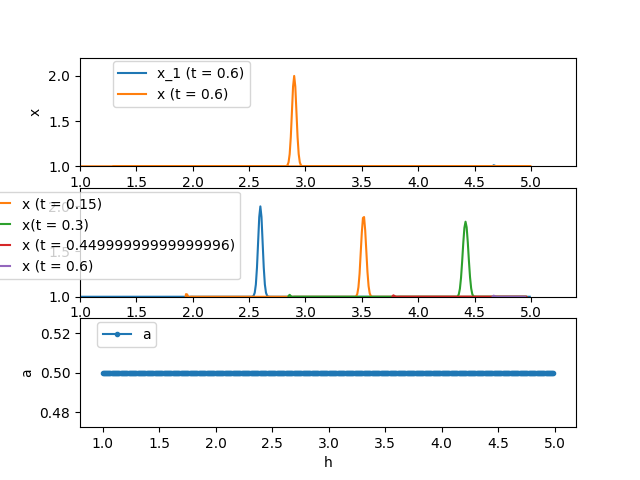
\includegraphics[width=1\linewidth]{tests_bcomp/a_const_x0_gauss.png} \\$a=const$}
    \end{subfigure}
    \begin{subfigure}{0.33\textwidth}
    {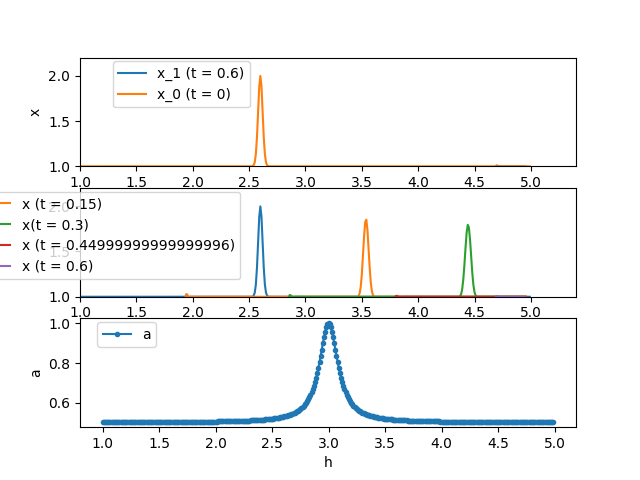
\includegraphics[width=1\linewidth]{tests_bcomp/a_hat_x0_gauss.png} \\$a - hat$}
    \end{subfigure}
    \begin{subfigure}{0.33\textwidth}
    {\includegraphics[width=1\linewidth]{tests_bcomp/a_tear_x0_gauss.png} \\$a - tear$}
    \end{subfigure}
\end{figure}
\begin{figure}[h]
    \caption{Пик}
    \begin{subfigure}{0.33\textwidth}
    {\includegraphics[width=1\linewidth]{tests_bcomp/a_const_x0_peak.png} \\$a=const$}
    \end{subfigure}
    \begin{subfigure}{0.33\textwidth}
    {\includegraphics[width=1\linewidth]{tests_bcomp/a_hat_x0_peak.png} \\$a - hat$}
    \end{subfigure}
    \begin{subfigure}{0.33\textwidth}
    {\includegraphics[width=1\linewidth]{tests_bcomp/a_tear_x0_peak.png} \\$a - tear$}
    \end{subfigure}
\end{figure}
\newpage
Заметим, что метод вносит достаточно сильное смещение, из-за которого иногда невозможно оценить результат его работы на исследуемом интервале координат и заданном временном отрезке. Также заметим, что изменение характера скорости переноса ($a$) слабо влияет на вид выходного сигнала, но при этом наименьшие искажения вносит константа.
Исходя из результатов тестов, данный метод благоприятен при решении задач, где необходимо моделировать распространение длинных и средних волн, при этом подавляя распространение высокочастотных гармоник. т.к. в этих случаях он вносит наименьшие искажения (\cite{bcomp},(24),(25)).


\subsection{Компактная схема}

Рассматривается задача Коши вида:
$$  \left\{
        \begin{array}{l}
            u_t + a \cdot u_x = 0, \: -\infty < x < \infty \\
            u(x,0) = u_0(x), \: x \ge 0
        \end{array}
    \right. $$

Рассмотрим задачу построения явной разностной схемы порядка аппроксимации $O(\tau) + O(h^k), \: k \ge 1$.

В компактных аппроксимациях используются небольшие сеточные шаблоны вдоль оси $x$. За счет привлечения таких же небольших шаблонов вдоль оси $x$ на верхнем, $(n + 1)$-ом слое по $t$ возникают дополнительные неопределенные коэффициенты при построении аппроксимации производной $u_x$. Распоряжаясь этими дополнительными коэффициентами, можно повысить порядок аппроксимации схемы. Для примера осуществим построение компактной разностной аппроксимации порядка $O(h^3)$ производной $u_x$. При этом предполагаем, что $u(x) \in C^4[a, b]$, где $[a, b]$ – промежуток на оси $x$, в котором задана функция $u(x)$. Пусть \begin{equation}
\label{eq_one}
    f(x) = u_x,
\end{equation}
$$ f_j = f(x_j), $$
$$ x_j = a + ( j - 1 ) \cdot h, $$
$$ h = \frac{ b - a }{ N - 1 }, \: N > 2. $$

Компактная апроксимация соотношения (\ref{eq_one}) может быть записана следующим образом:
\begin{equation}
\label{eq_two}
    \alpha f_{j-1} + \beta f_j + \gamma f_{j+1} = \frac{u_j-u_{j-1}}{h}.
\end{equation}

Подбираем неопределённые коэффициенты $\alpha$, $\beta$ и $\gamma$ с учётом соотношения:
\begin{equation}
\label{eq_three}
    \left| \alpha f_{j-1} + \beta f_j + \gamma f_{j+1} - \frac{u_j-u_{j-1}}{h} \right| = O(h^3)
\end{equation}

Подставим в (\ref{eq_two}) разложения в ряды Тейлора функций $f(x)$ и $u(x)$ в точке $x = x_j$:
$$  \alpha \left( f_j - h f^{(1)}_x + \frac{h^2}{2} f^{(2)}_x - \frac{h^3}{6} f^{(3)}_x + \frac{h^4}{24} f^{(4)}_x \right) + \beta f_j + \gamma \left( f_j + h f_x + \frac{h^2}{2} f^{(2)}_x + \frac{h^3}{6} f^{(3)}_x + \frac{h^4}{24} f^{(4)}_x \right) = $$
$$  {} = \frac{1}{h} \left( u_j - u_j + h u^{(1)}_x + \frac{h^2}{2} u^{(2)}_x + \frac{h^3}{6} u^{(3)}_x + \frac{h^4}{24} u^{(4)}_x \right) + O(h^4) $$

Учтем тот факт, что $f = \frac{du}{dx}$. В результате получим следующее уравнение:
\begin{equation}
\label{eq_four}
    \left( \alpha + \beta + \gamma \right) \cdot f_j+  h \cdot \left( \gamma - \alpha + \frac{1}{2} \right) \cdot f^{(1)}_x + h^2 \cdot \left[ \frac{1}{2} ( \alpha + \beta ) - \frac{1}{6}\right] \cdot f^{(2)}_x + h^3 \cdot \left[ \frac{1}{6} ( \gamma  - \alpha ) - \frac{1}{24} \right] \cdot f^{(3)}_x = O(h^4)
\end{equation}

Для того, чтобы это соотношение выполнялось при любой функции $f(x) \in C^3[a,b]$ и, кроме того, выполнялось условие (\ref{eq_three}), потребуем, чтобы пока неопределенные коэффициенты $\alpha$, $\beta$, $\gamma$ удовлетворяли системе:
$$  \left\{
        \begin{array}{l}
            \alpha + \beta + \gamma = 1 \\
            \gamma - \alpha + \frac{1}{2} = 0 \\
            \frac{ ( \alpha + \gamma ) }{2} - \frac{1}{6} = 0
        \end{array}
    \right. $$

Решая эту систему, получим:
$$\alpha=\frac{5}{12}, \: \beta=\frac{8}{12}, \: \gamma=-\frac{1}{12}.$$

Подставляя найденные значения в (2), получим с учетом (4):
\begin{equation}
\label{eq_five}
    \frac{5}{12}f_{j-1}+\frac{8}{12}f_j-\frac{1}{12}f_{j+1}=\frac{u_j-u_{j-1}}{h}+\frac{h^3}{24}f_{xxx}+O(h^4).
\end{equation}

Из (\ref{eq_five}) следует, что если $u(x) \in C^4[a, b]$, то выполняется оценка (\ref{eq_three}). Введем разностный оператор $A$ по формуле:
$$ A f_{j-1} = \frac{5}{12} f_{j-1} + \frac{8}{12} f_j - \frac{1}{12} f_{j+1}.$$

Перепишем в виде:
$$ A f_j = \frac{ u_j - u_{j-1} }{h}.$$

Здесь мы опустили члены высокого порядка малости $O(h^3) + O(h^4)$. Отсюда получаем следующую компактную аппроксимацию производной $f_j = du(x_j)/dx$ третьего порядка точности:
$$f_j=A^{-1}(\frac{u_j-u_{j-1}}{h}).$$

Теперь на основе это построим простейшую двухслойную компактную разностную схему порядка аппроксимации $O(\tau) + O(h^3)$ для уравнения  задачи Коши при $\alpha > 0$:
$$A\frac{u^{n+1}_j-u^n_j}{\tau}+\alpha[\sigma\frac{u^{n+1}_j-u^{n+1}_{j-1}}{h}+(1-\sigma)\frac{u^n_j-u^n_{j-1}}{h}]=0. $$

Здесь $\sigma$ – весовой множитель, $0 \le \sigma \le 1$. Подействовали на обе части оператором А. В результате получили окончательный вид однопараметрического семейства компактных разностных схем. Схема имеет порядок аппроксимации $O(\tau^2) + O(h^3)$ при $\sigma = 0.5$ и порядок $O(\tau) + O(h^3)$ при $\sigma \not= 0.5$ и является абсолютно устойчивой при $\sigma \ge 0.5$.


\begin{thebibliography}{99}

\bibitem{vor} Е. В. ВОРОЖЦОВ. СБОРНИК ЗАДАЧ ПО ТЕОРИИ РАЗНОСТНЫХ СХЕМ. Новосибирск 2000

\bibitem{an_effective} Yanjie Zhou, Dinghui Yang, Xiao Ma, Jingshuang Li 2015 An effective method to suppress numerical dispersion in 2D acoustic and elastic modelling using a high-order Padé approximation 

\bibitem{finite} Randall J. LeVeque 2004 Finite Volume Methods for Hyperbolic Problems

\bibitem{free_and_smooth} B. Lombard, J. Piraux, C. Gélis and J. Virieux 2007 Free and smooth boundaries in 2-D finite-difference schemes for transient elastic waves Geophys. J. Int. (2008) 172, 252–261

\bibitem{chel} Челноков Ф. Б. 2005 Численное моделирование деформационных динамических процессов в средах со сложной структурой

\bibitem{garvin} W. W. Garvin 1956 Exact Transient Solution of the Buried Line Source Problem

\bibitem{bcomp} МОНОТОННАЯ ВЫСОКОТОЧНАЯ КОМПАКТНАЯ СХЕМА БЕГУЩЕГО СЧЕТА ДЛЯ КВАЗИЛИНЕЙНЫХ УРАВНЕНИЙ ГИПЕРБОЛИЧЕСКОГО ТИПА", Б.В. Рогов, М.Н. Михайловская

\bibitem{2.5D} 2.5-dimensional crosshole acoustic response: a variable density approach, J. P. Narayan, Geophys J Int (1999) 139 (3): 879-887.

\bibitem{manuscript} A pressure-based semi-implicit space-time discontinuous Galerkin method on staggered unstructured meshes for the solution of the compressible Navier-Stokes equations at all Mach numbers, Maurizio Tavelli, Michael Dumbser, Journal of Computational Physics, 15 July 2017, Pages 341–376

\bibitem{weno} S.V. Mikhaylov (TsAGI), A.A. Saveliev (TsAGI), Tran Dinh Thang (MIPT), Nguyen Ngoc Sang (MIPT)
Using WENO method in framework of ZEUS architecture

\bibitem{weno5d} А.Н.Кудрявцев СОВРЕМЕННЫЕ ЧИСЛЕННЫЕ МЕТОДЫ
СВЕРХЗВУКОВОЙ АЭРОДИНАМИКИ Новосибирский государственный университет, 2003–2014 гг.

\bibitem{petrov}  М.Н.Петров МОДЕЛИРОВАНИЕ СЕЙСМИЧЕСКИХ ВОЛН, ВЫЗВАННЫХ УДАРОМ МЕТЕОРИТА

\bibitem{clawpack} HIGH-ORDER WAVE PROPAGATION ALGORITHMS FOR HYPERBOLIC SYSTEMS
DAVID I. KETCHESON, MATTEO PARSANI, AND RANDALL J. LEVEQUE

Mach numbers
\end{thebibliography}


\end{document}